\section{Качество переходных процессов}

Рассмотрим систему, заданную передаточной функцией:
\begin{eqnarray}
    W(s) = \frac{\lambda_1\lambda_2\lambda3}{(s-\lambda_1)(s-\lambda_2)(s-\lambda_3)}
\end{eqnarray}

\subsection{Корневые критерии качества}
Оценить характер переходного процесса можно по корням характеристического уравнения, они 
же являются полюсами передаточной функции. В случае приближенной оценки качества, на 
комплексной плоскости, на которой расположены корни характеристического уравнения 
отмечается трапециевидная область, внутри которой находятся все корни. 

Время переходного процесса $T$ зависит от максимальной величины действительной части 
корней характеристического уравнения, то есть отдалением правой границы трапеции от 
мнимой оси. Чем больше это расстояние, тем меньше время переходного процесса. 
\begin{equation}
    T \approx \frac{1}{|\text{max}(Re(\lambda))|}
\end{equation}

Перерегулирование $\sigma$ зависит от колебательности системы, которая пропорциональна значению:
\begin{eqnarray}
    \mu = \text{max}\left|\frac{Im(\lambda)}{Re(\lambda)}\right|
\end{eqnarray}
или же тангенсу угла наклона стороны трапеции. 

\FloatBarrier
\subsection{Сравнение систем}
Будем поочередно рассматривать разные комбинации коэффициентов $\lambda_1$, $\lambda_2$, $\lambda_3$ 
и оценивать переходный процесс по времени переходного процесса $T$ и перерегулированию $\sigma$. 
Будем считать, что переходный процесс завершился, когда значение выходной величины
зашло в окрестность установившегося значения и более не выходит из нее. В качестве допустимого 
отклонения от целевого значения возьмем $0.1$.
Конечные результаты занесены в таблицу \ref{tab:quality}. 

\subsubsection{Эксперемент 1}
\label{task2_case1}

Для начала выберем коэффициенты $\lambda_1 = \lambda_2 = \lambda_3 = -3$. Расположение корней 
на комплексной плоскости и результаты моделирования системы приведены на 
рисунках \ref{fig:task_2_points1} и \ref{fig:task_2_case1}. 

Заметим, что в данном случае значение $\mu$ равно нулю, таким образом, перерегулирование
отсутствует. При этом время переходного процесса составило 2.45 секунды.

\begin{figure}
    \centering
    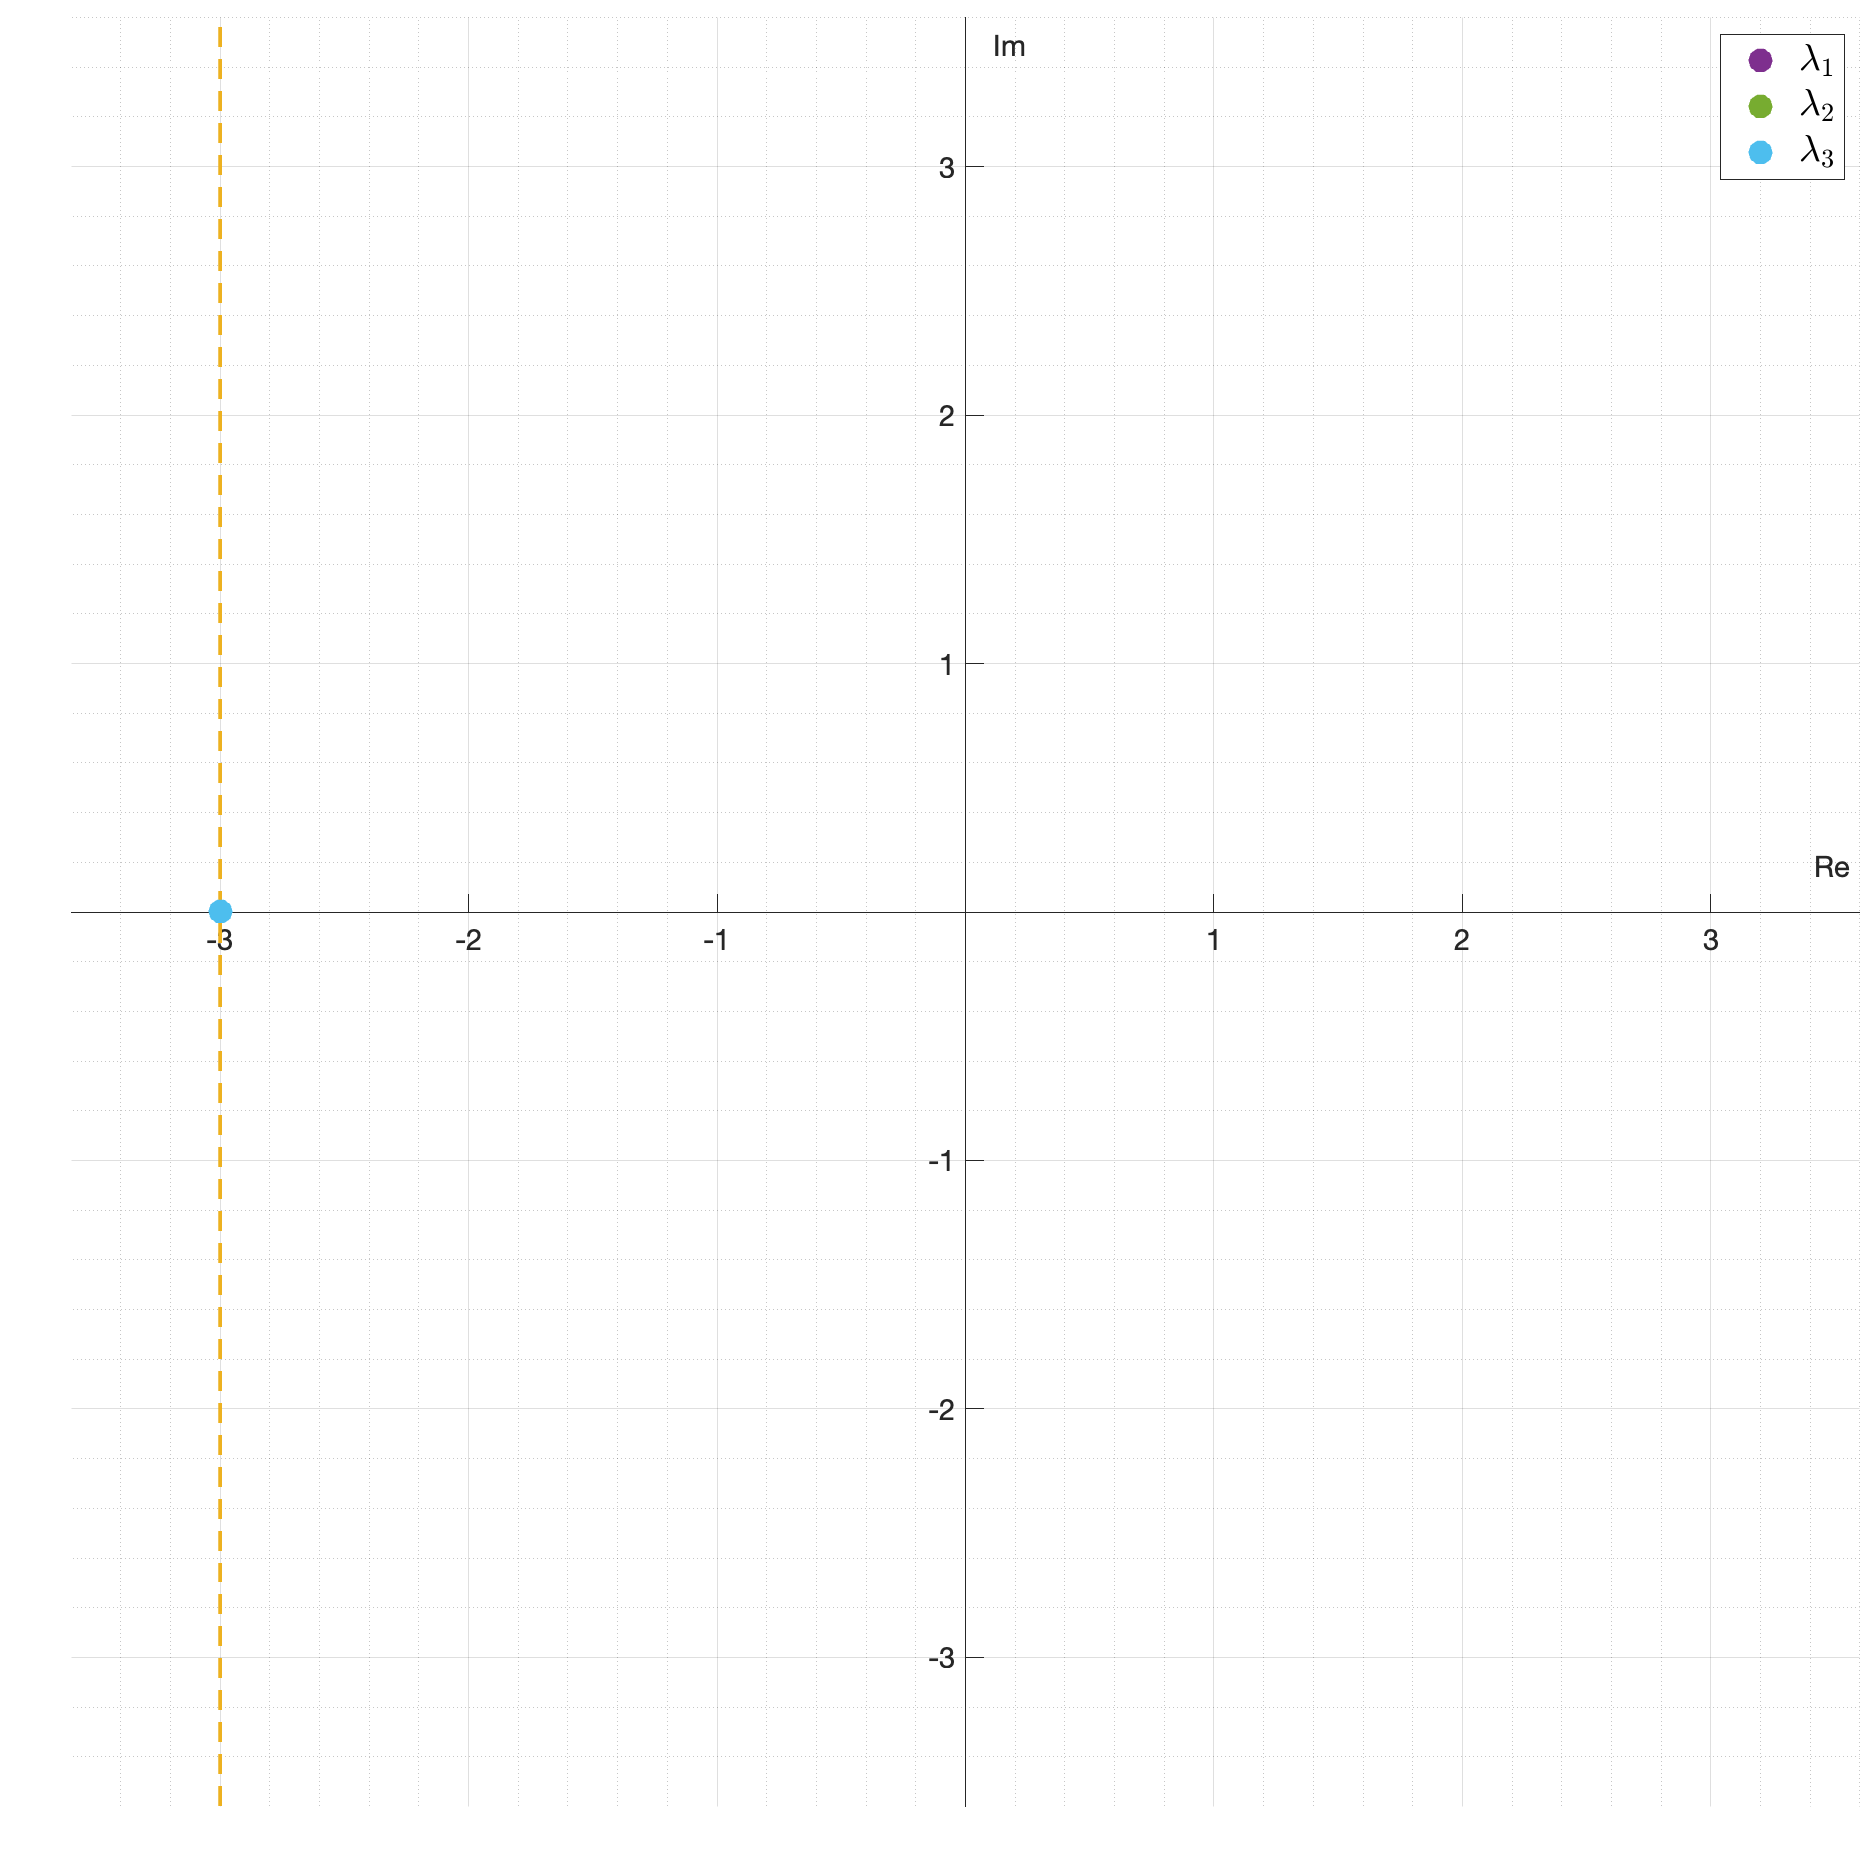
\includegraphics[width=0.8\textwidth]{media/plots/task2_points1.png}
    \caption{Расположение корней на комплексной плоскости в эксперименте 1}
    \label{fig:task_2_points1}
\end{figure}

\begin{figure}
    \centering
    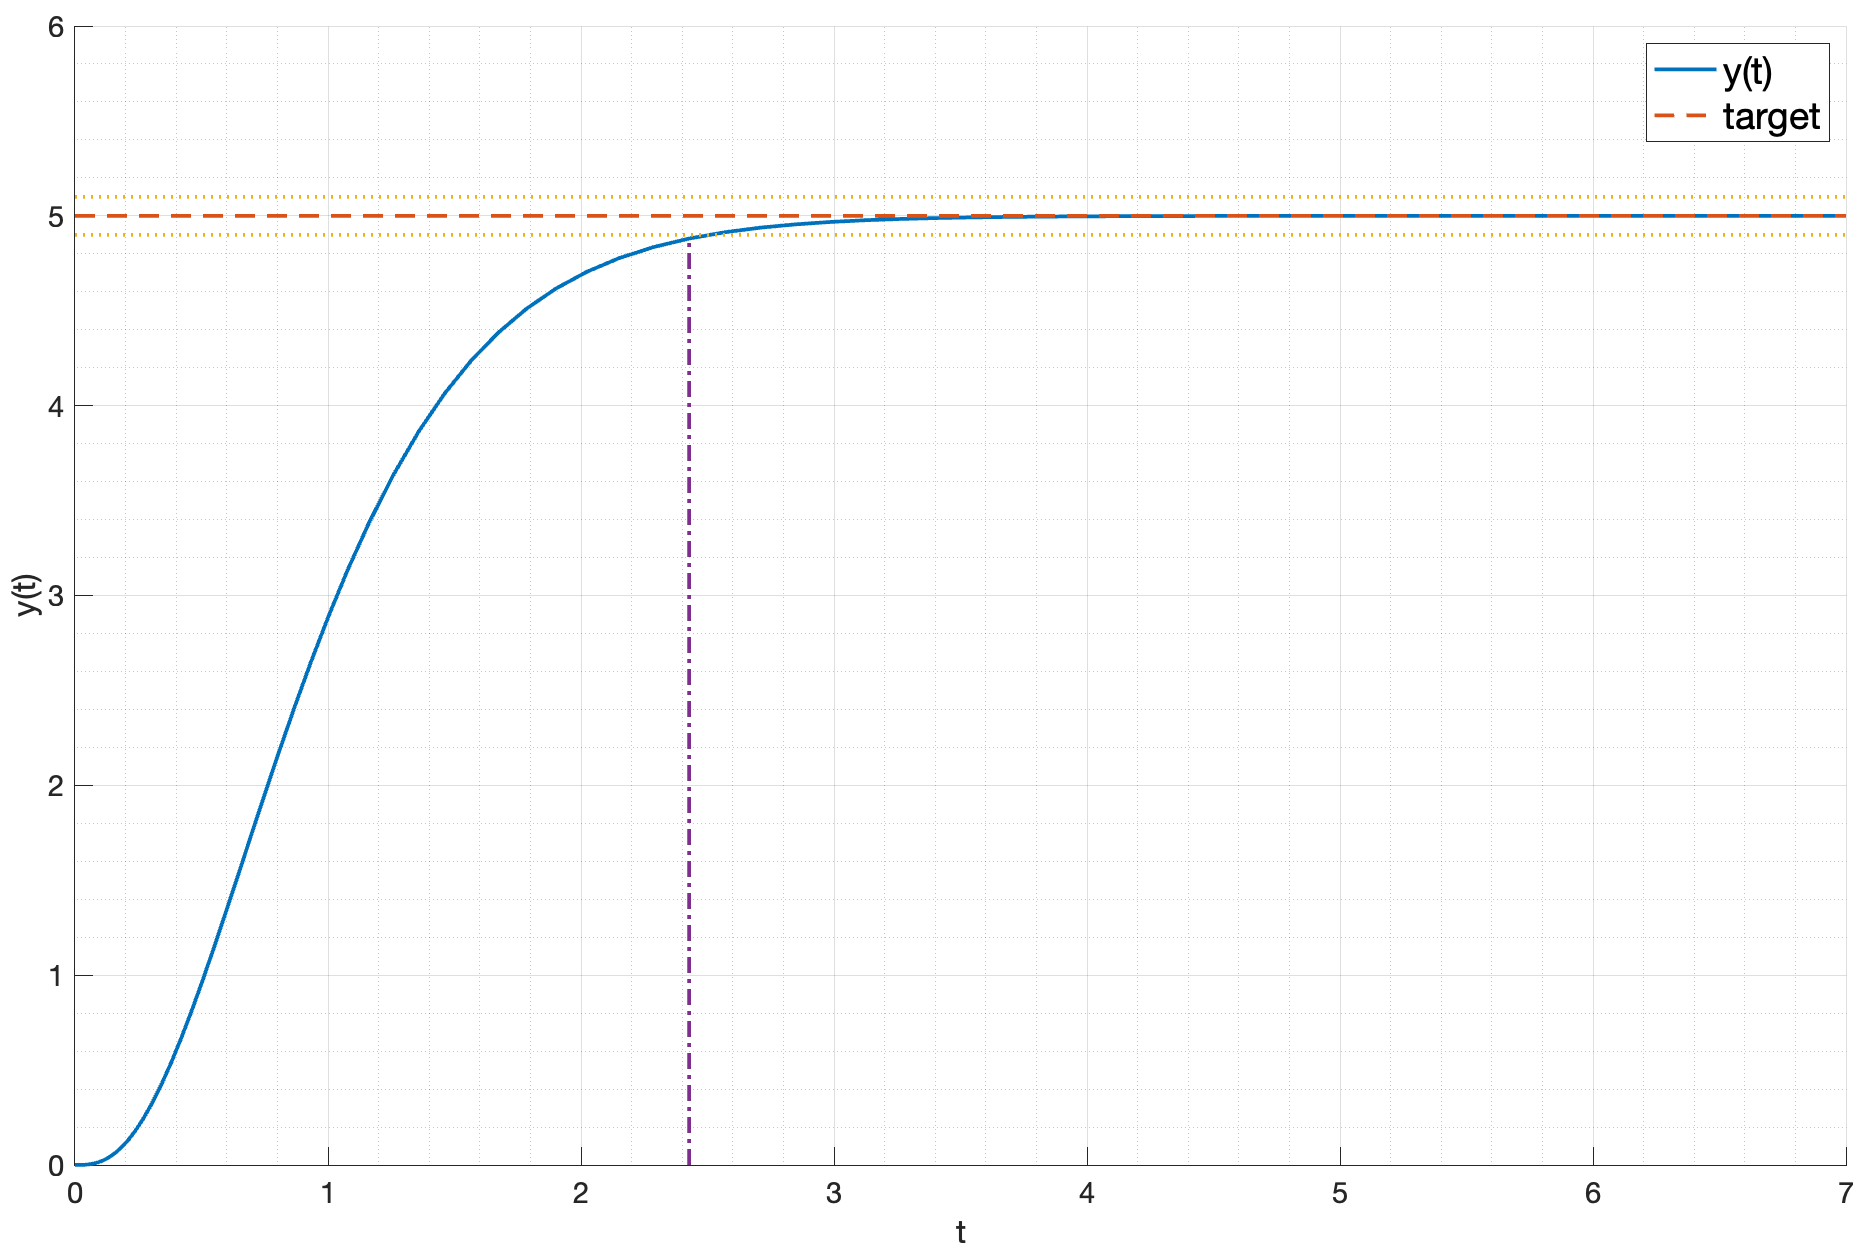
\includegraphics[width=\textwidth]{media/plots/task2_case1.png}
    \caption{Моделирование системы в эксперименте 1}
    \label{fig:task_2_case1}
\end{figure}

\subsubsection{Эксперемент 2}
\label{task2_case2}

Теперь изменим значение одного коэффициента на меньшее. Рассмотрим набор 
$\lambda_1 = -5$, $\lambda_2 = -3$, $\lambda_3 = -3$. Расположение корней 
и результаты моделирования приведены на рисунках \ref{fig:task_2_points2} и
\ref{fig:task_2_case2}.

\begin{figure}
    \centering
    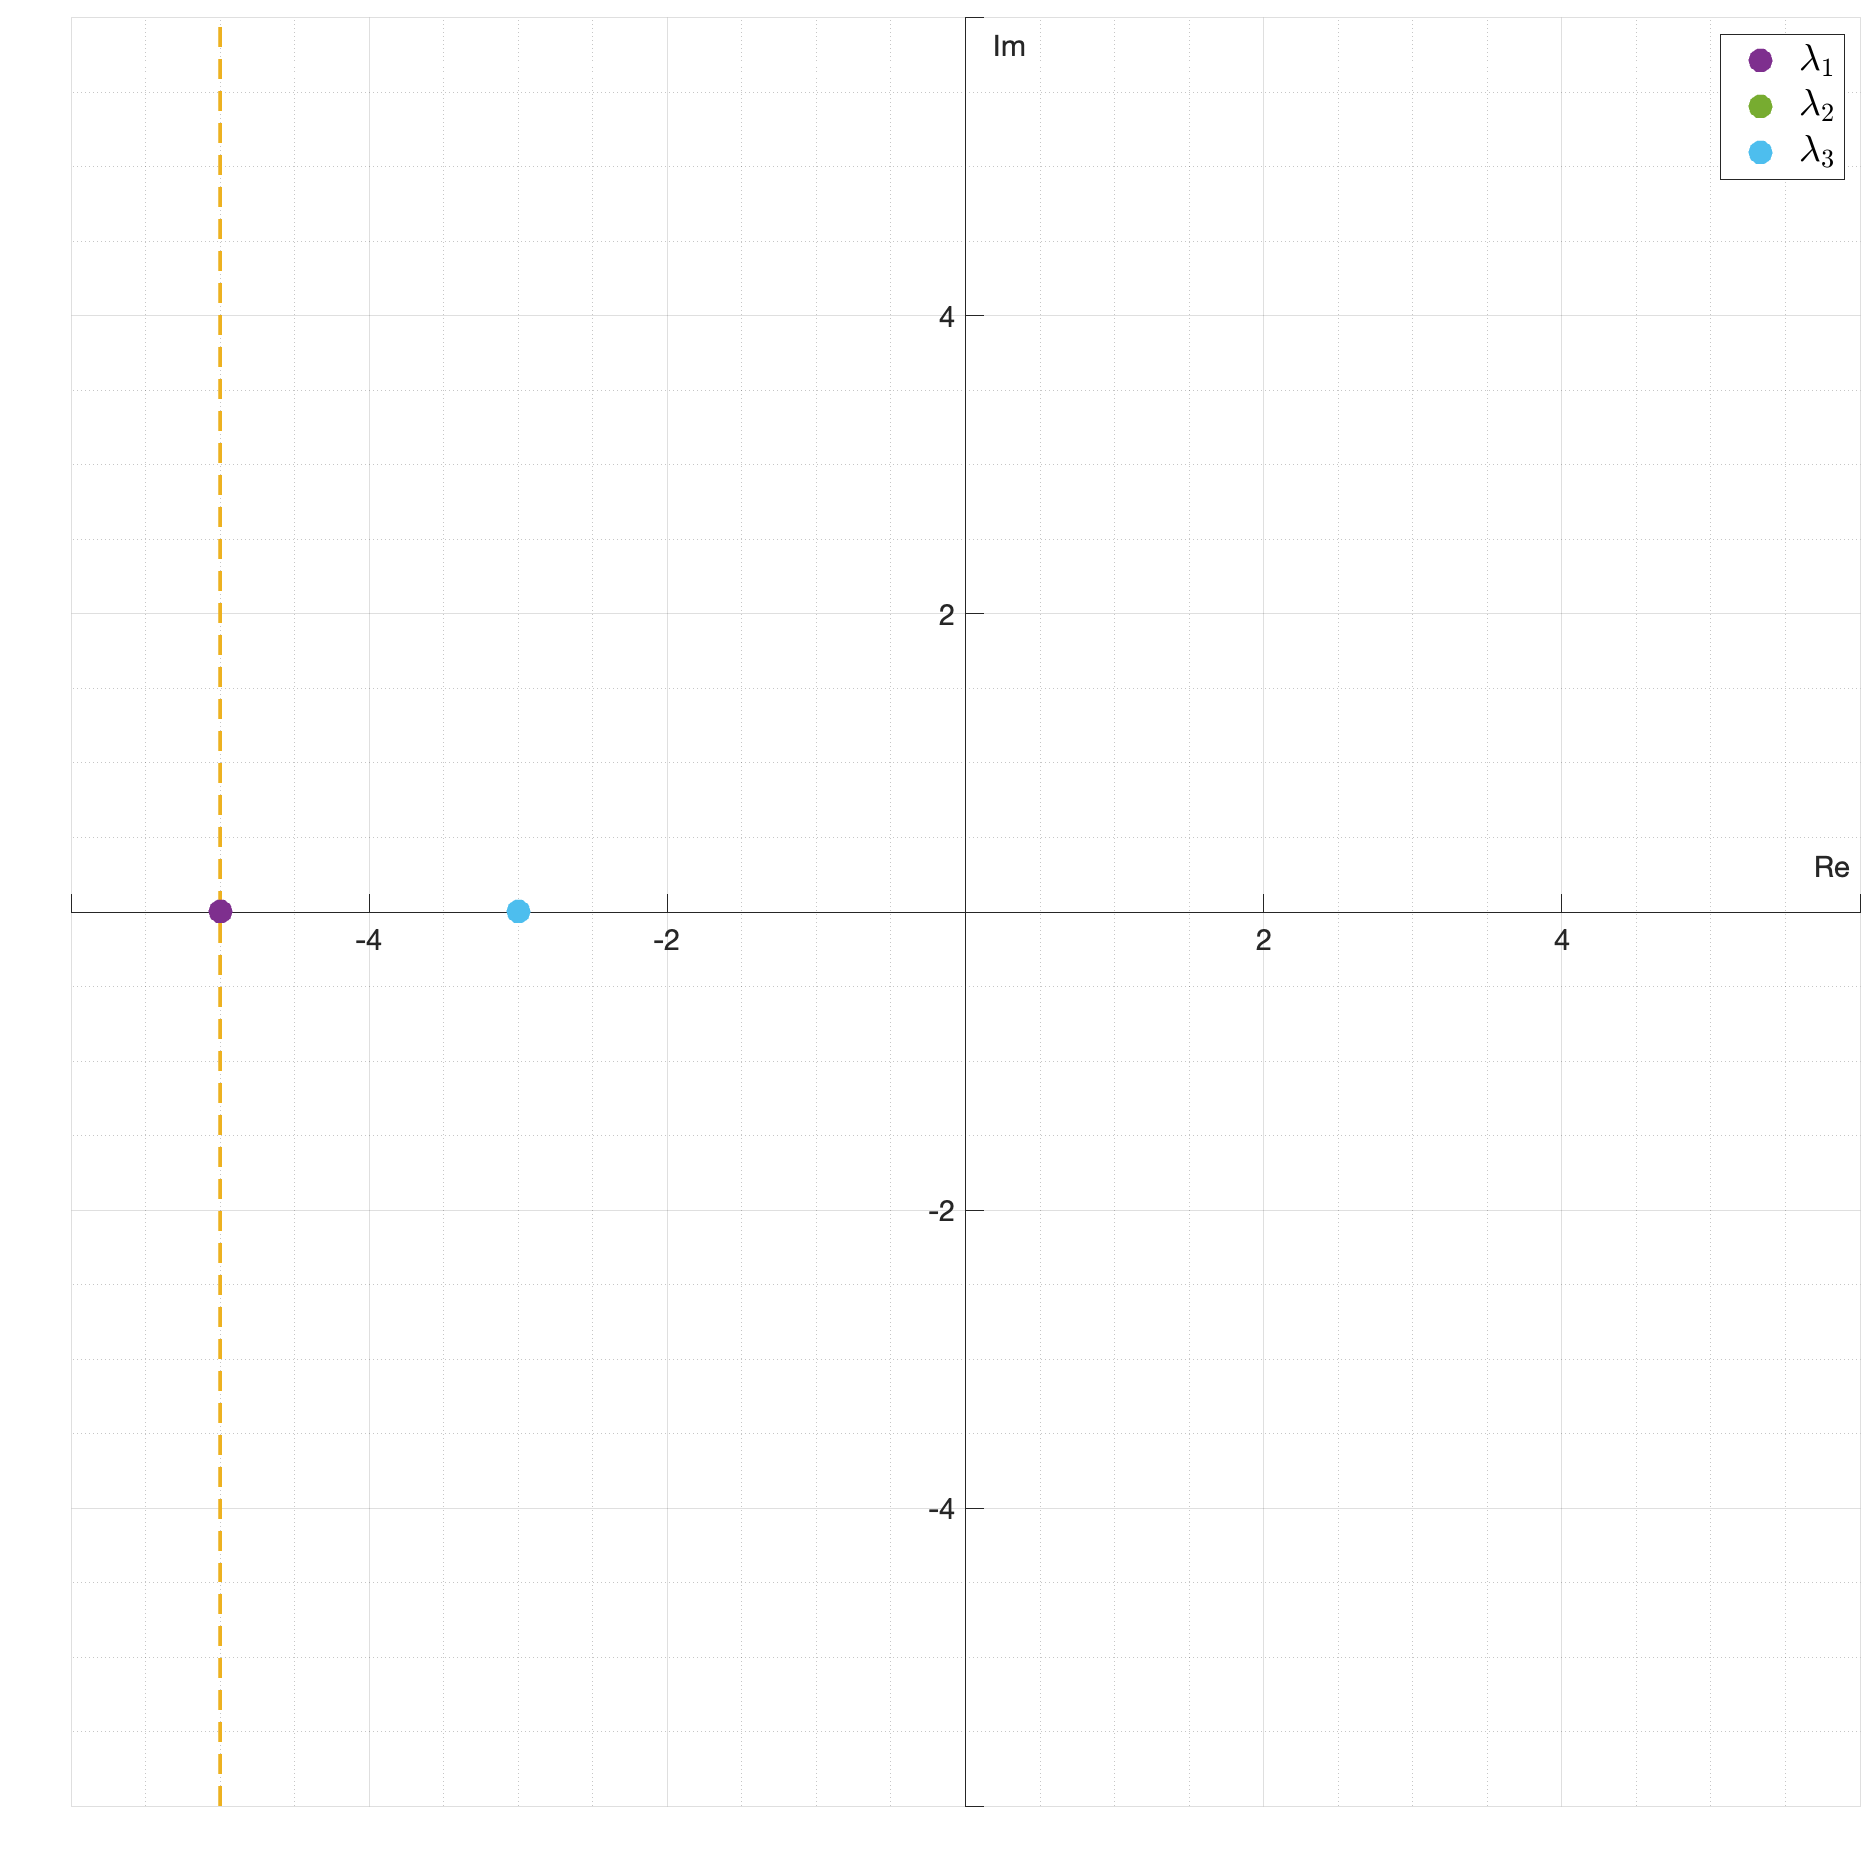
\includegraphics[width=0.8\textwidth]{media/plots/task2_points2.png}
    \caption{Расположение корней на комплексной плоскости в эксперименте 2}
    \label{fig:task_2_points2}
\end{figure}

\begin{figure}
    \centering
    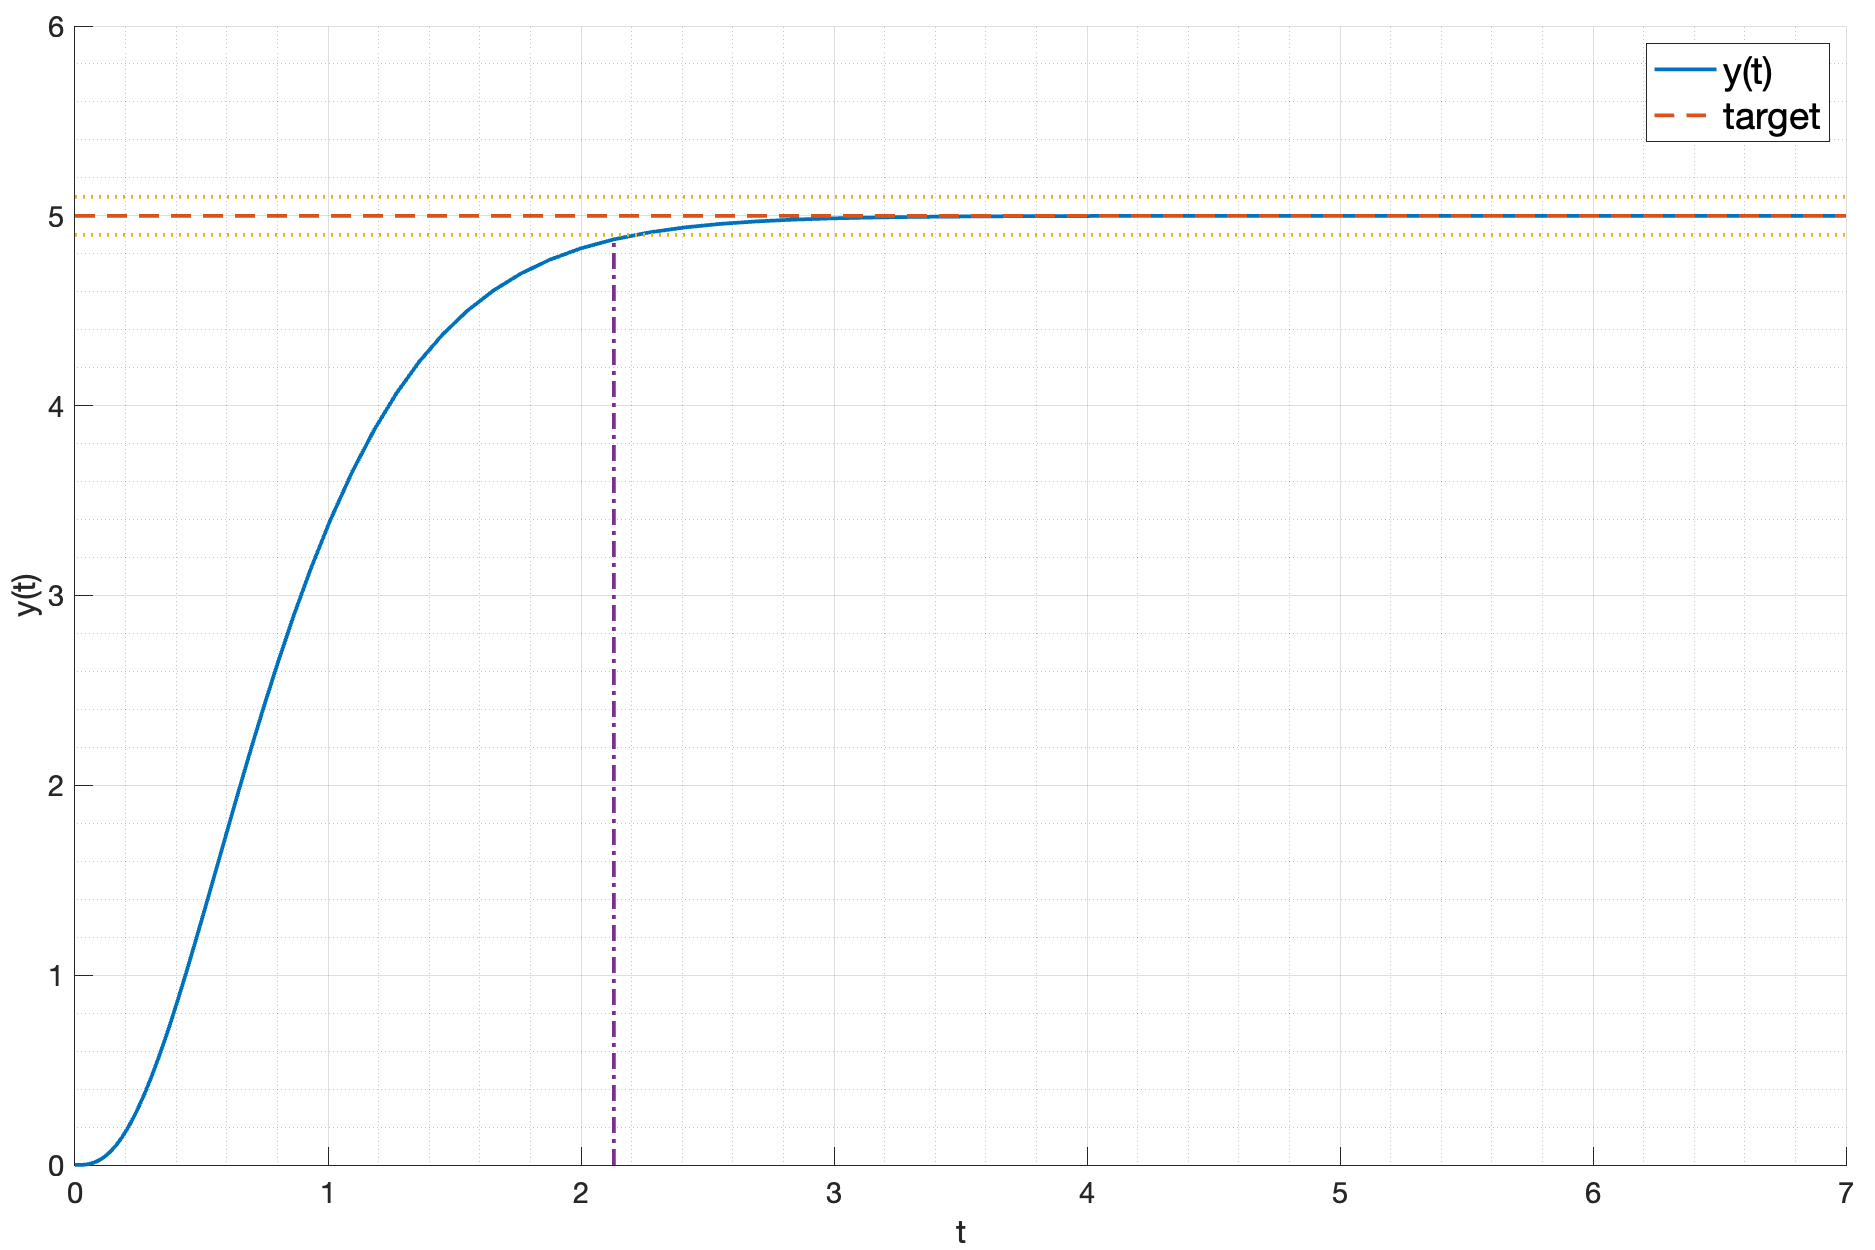
\includegraphics[width=\textwidth]{media/plots/task2_case2.png}
    \caption{Моделирование системы в эксперименте 2}
    \label{fig:task_2_case2}
\end{figure}

В данном случае так же нет перерегулирования из-за отсутствия мнимых корней.
Время переходного процесса составило 2.15 секунды, что несколько меньше, чем в предыдущем случае.

\subsubsection{Эксперемент 3}
\label{task2_case3}
Теперь уменьшим значения еще одного коэффициента. Рассмотрим набор 
$\lambda_1 = -5$, $\lambda_2 = -5$, $\lambda_3 = -3$. Расположение корней
и результаты моделирования приведены на рисунках \ref{fig:task_2_points3} и
\ref{fig:task_2_case3}.

\begin{figure}
    \centering
    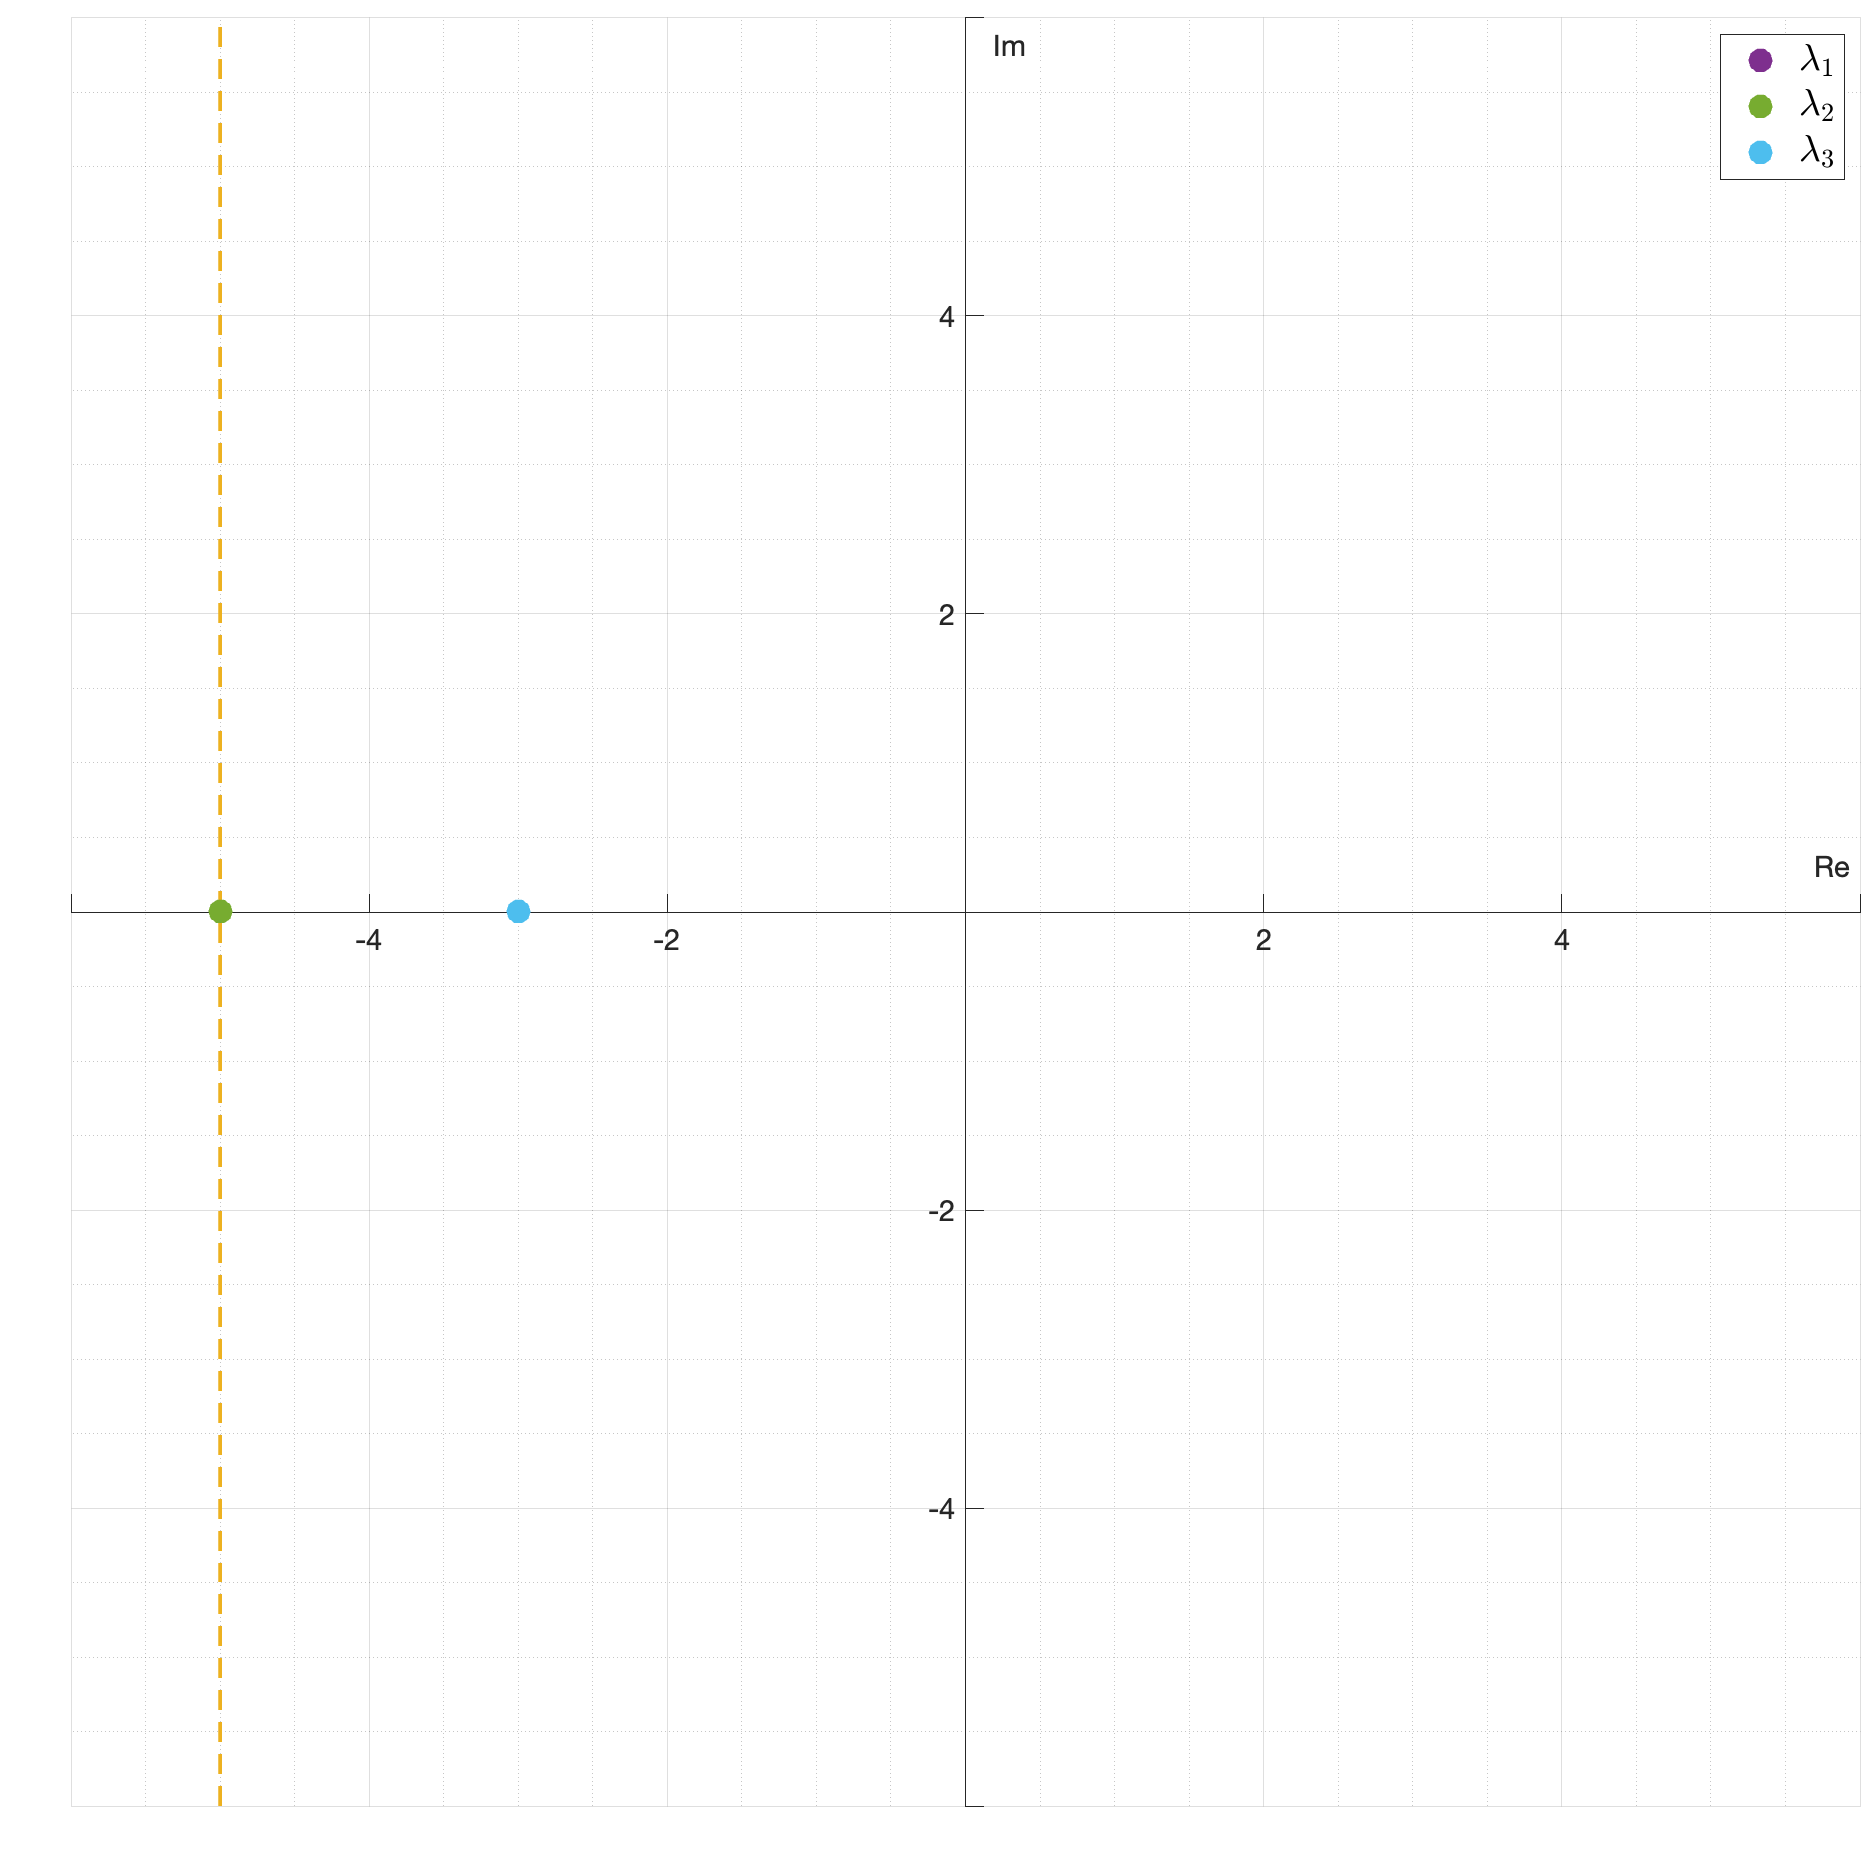
\includegraphics[width=0.8\textwidth]{media/plots/task2_points3.png}
    \caption{Расположение корней на комплексной плоскости в эксперименте 3}
    \label{fig:task_2_points3}
\end{figure}

\begin{figure}
    \centering
    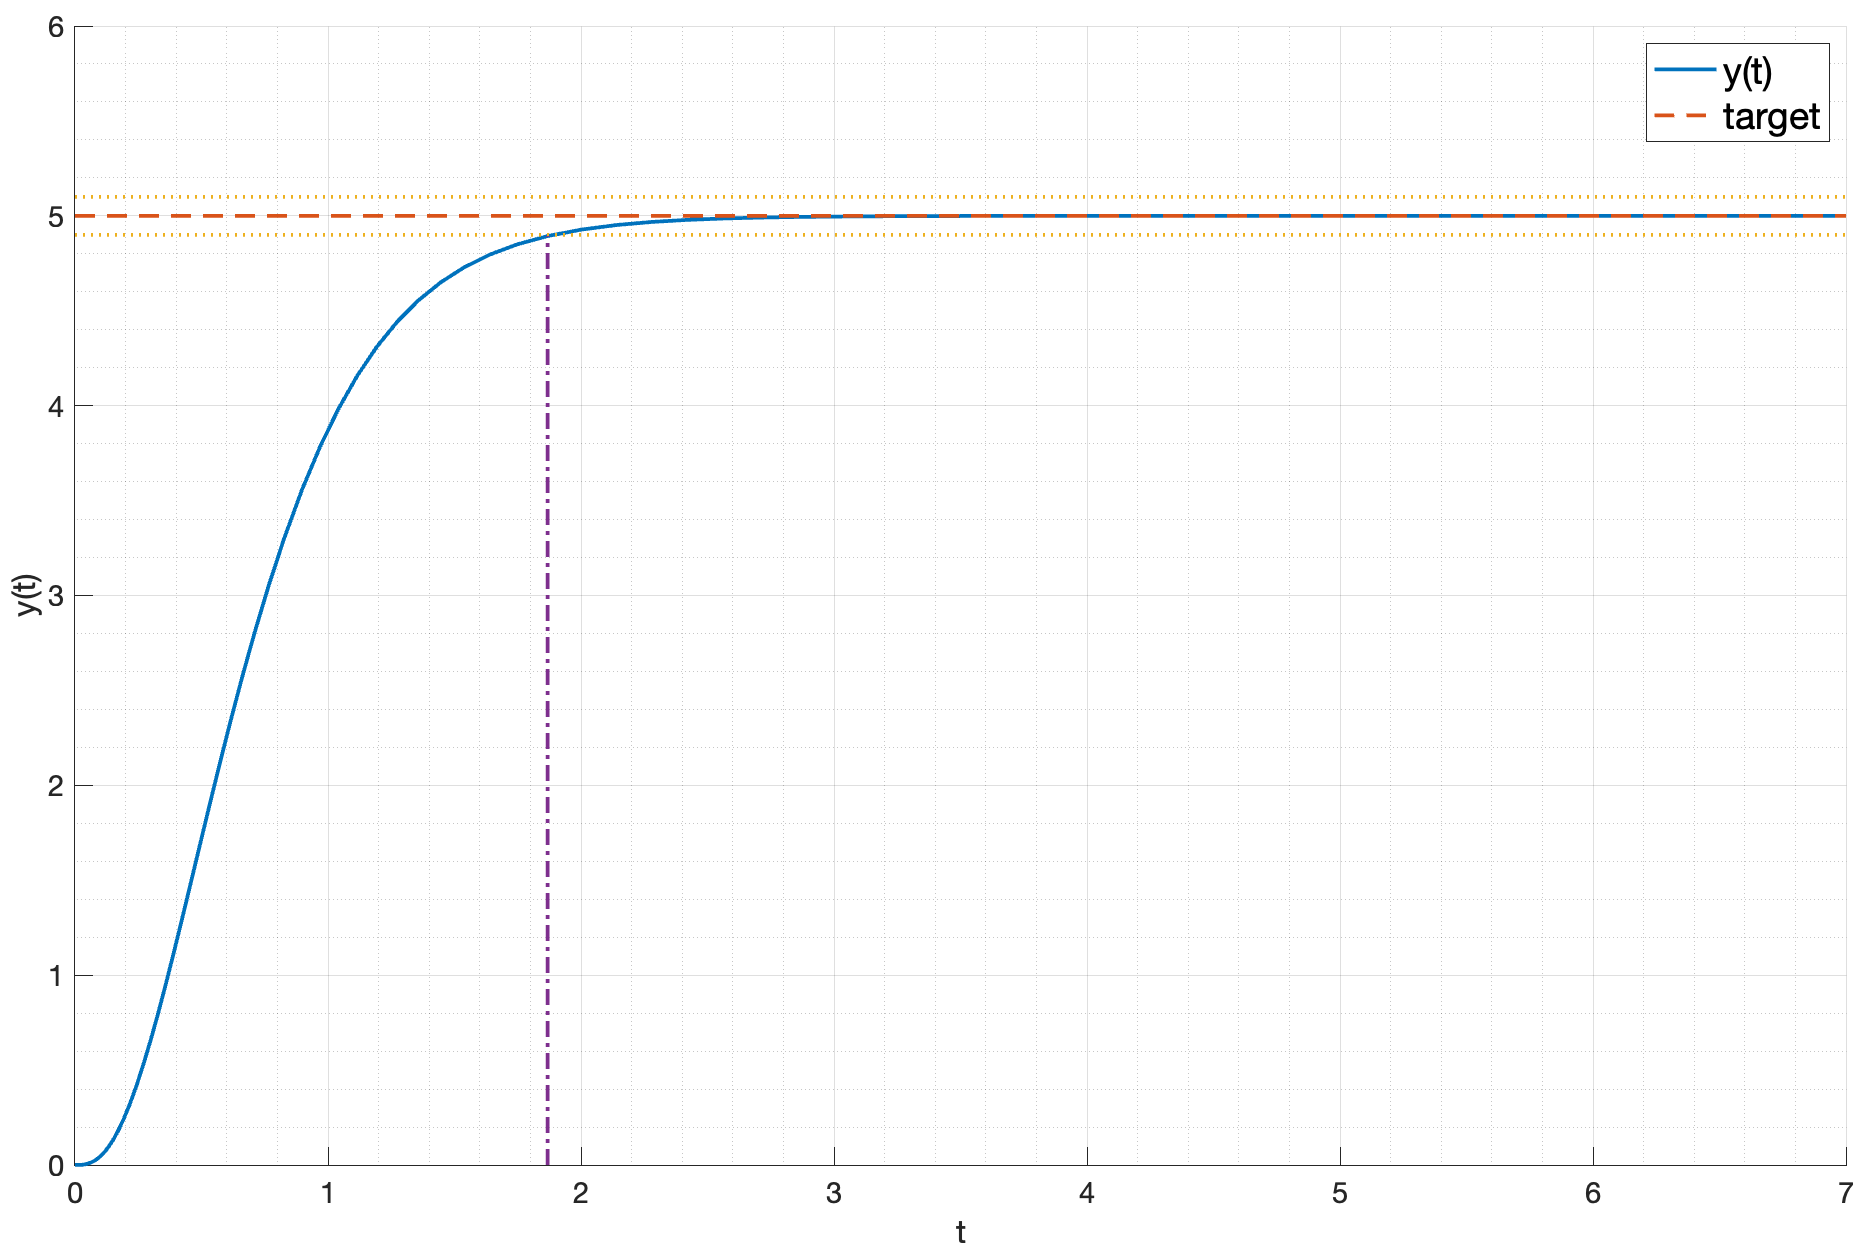
\includegraphics[width=\textwidth]{media/plots/task2_case3.png}
    \caption{Моделирование системы в эксперименте 3}
    \label{fig:task_2_case3}
\end{figure}

Время переходного процесса еще сильнее уменьшилось и составило 1.83 секунды. 

\subsubsection{Эксперемент 4}
\label{task2_case4}
Теперь увеличим значение одного коэффициента. Рассмотрим набор 
$\lambda_1 = -5$, $\lambda_2 = -5$, $\lambda_3 = -1$. 
Расположение корней и результаты моделирования приведены на рисунках 
\ref{fig:task_2_points4} и \ref{fig:task_2_case4}.

\begin{figure}
    \centering
    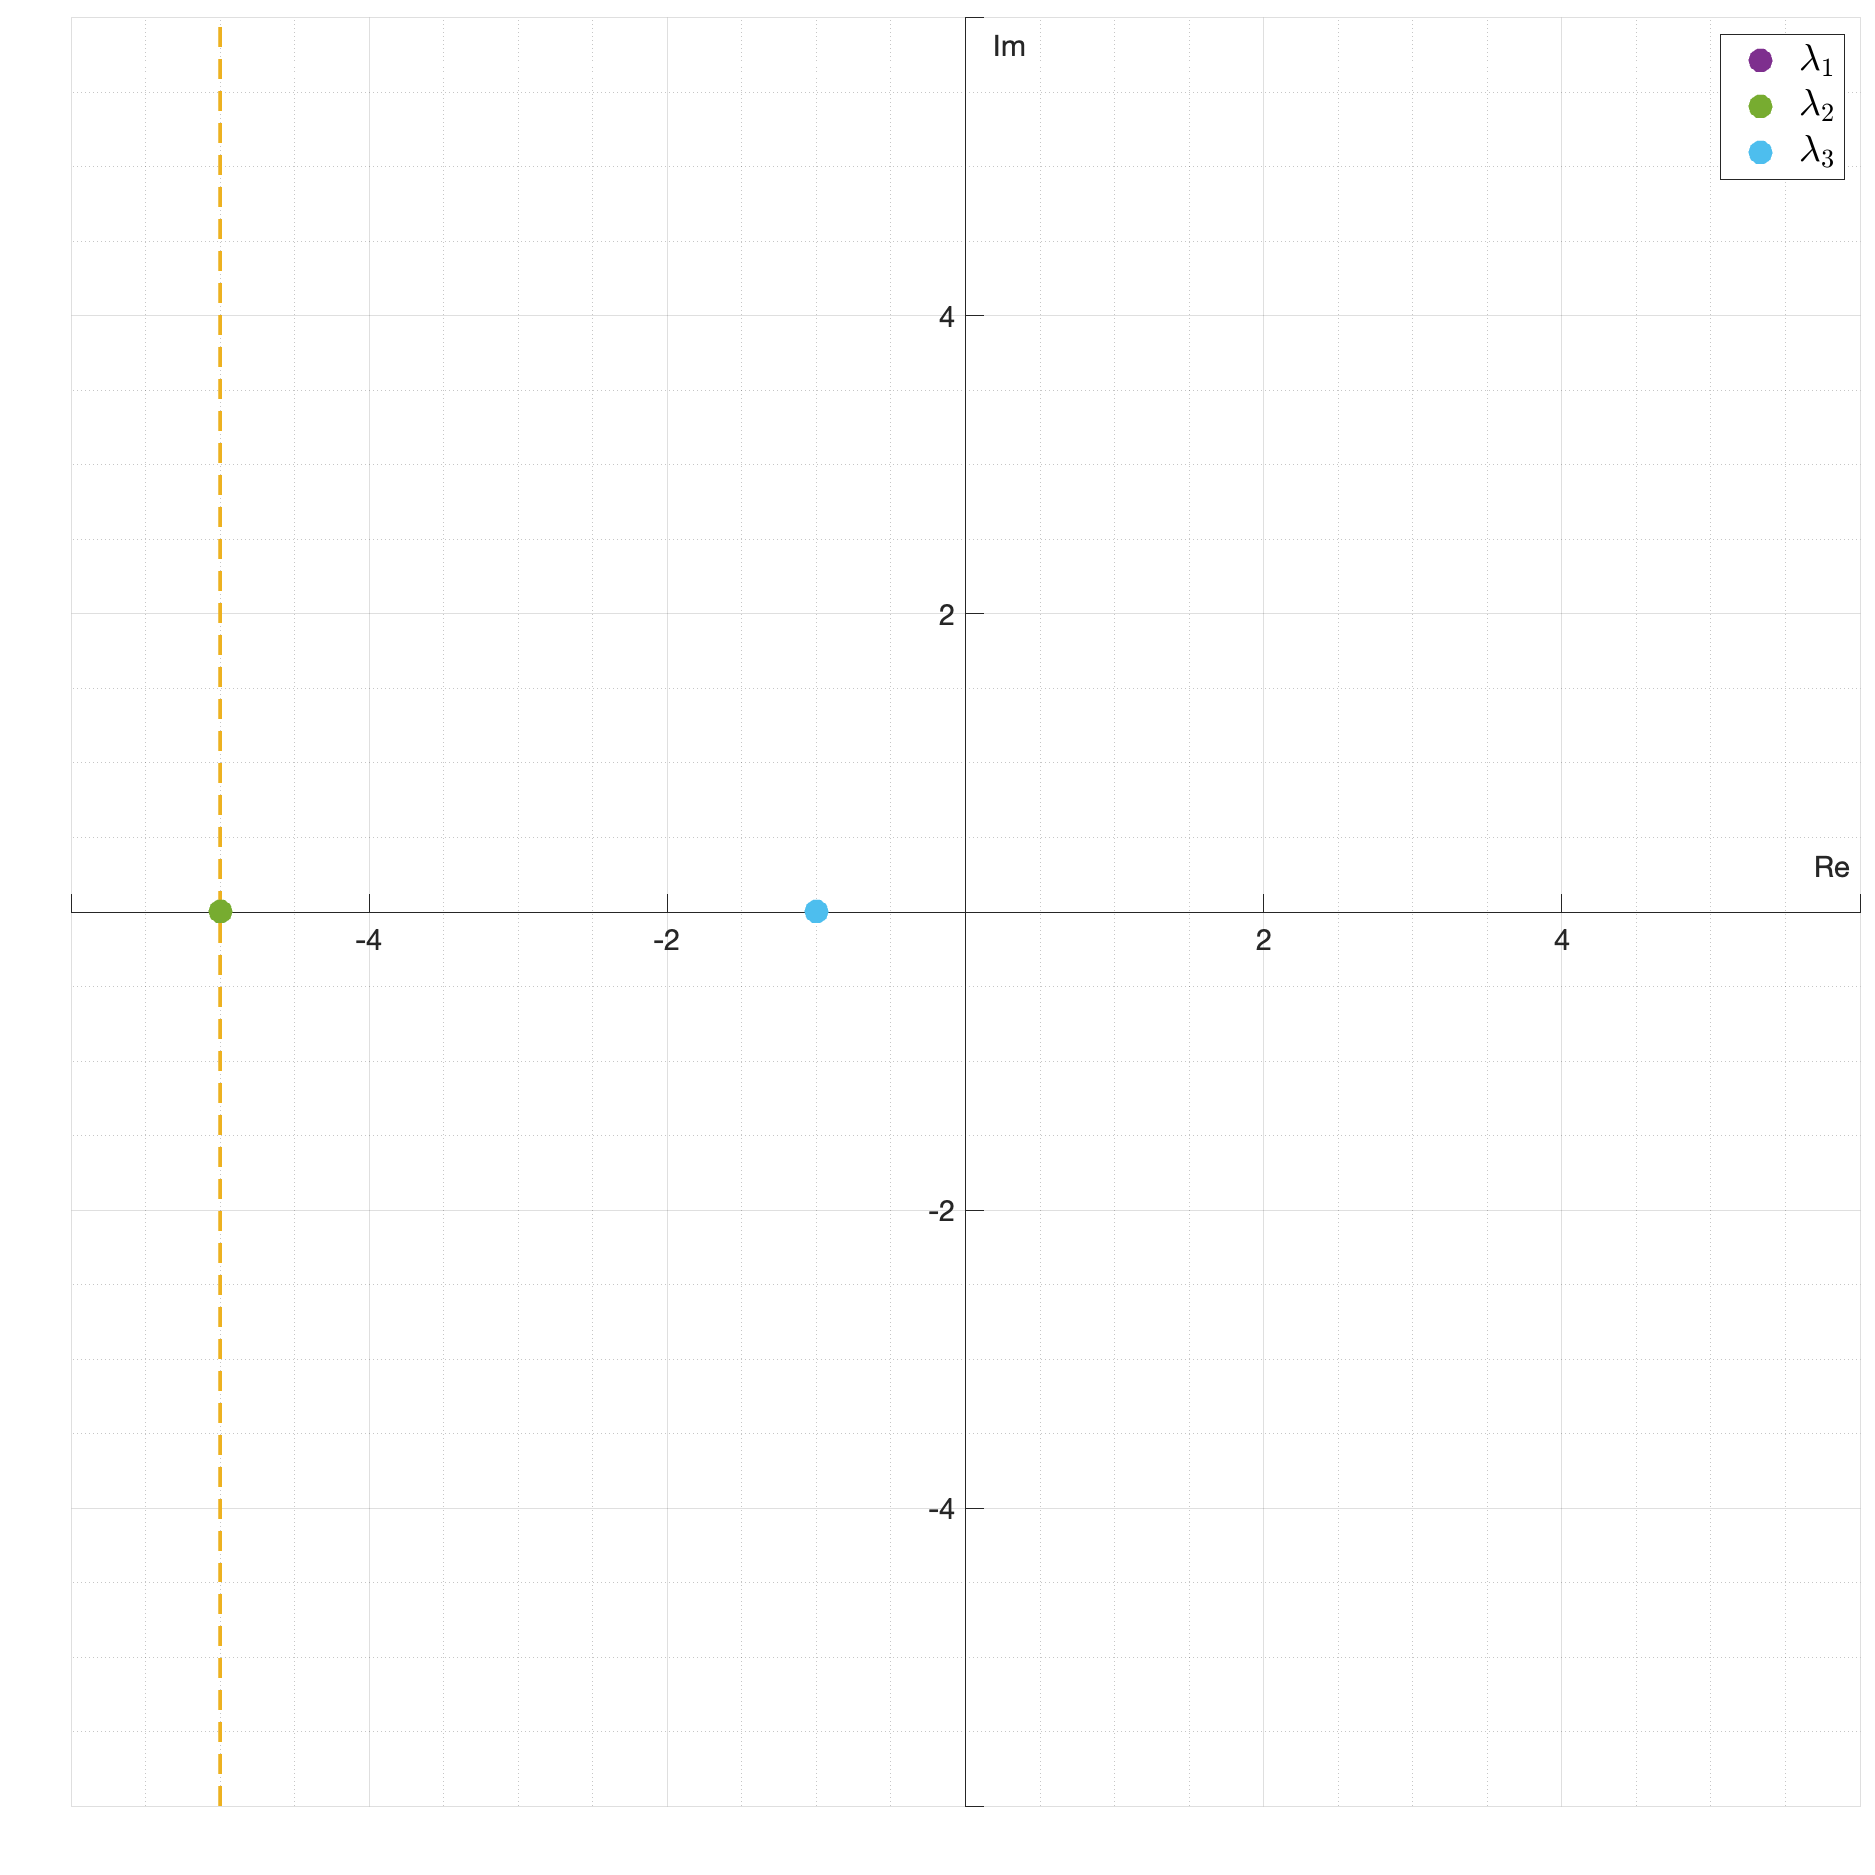
\includegraphics[width=0.8\textwidth]{media/plots/task2_points4.png}
    \caption{Расположение корней на комплексной плоскости в эксперименте 4}
    \label{fig:task_2_points4}
\end{figure}

\begin{figure}
    \centering
    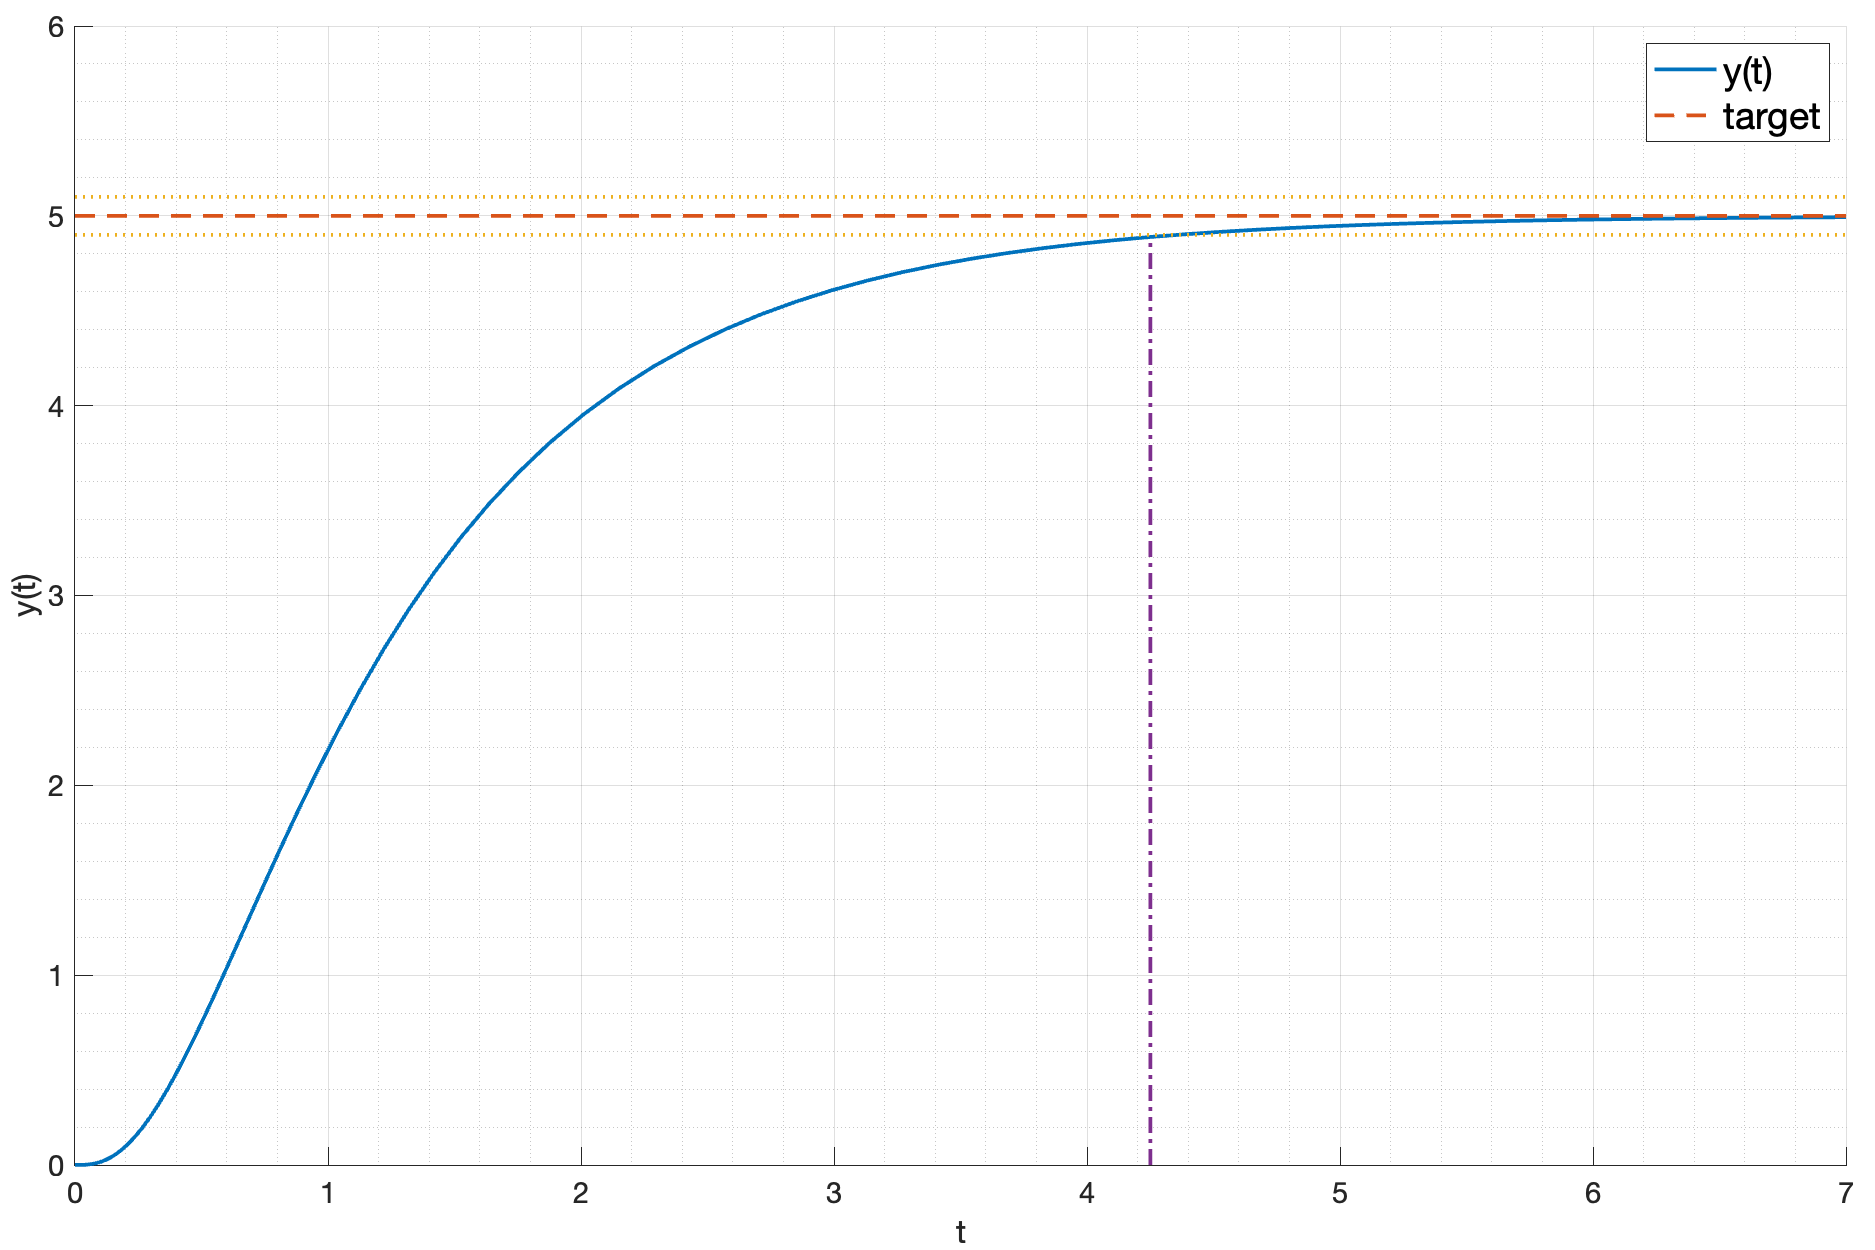
\includegraphics[width=\textwidth]{media/plots/task2_case4.png}
    \caption{Моделирование системы в эксперименте 4}
    \label{fig:task_2_case4}
\end{figure}

Видно, что время переходного процесса увеличилось до 4.31 секунды. При таком же по модулю 
изменению корня, но в другую сторону, время переходного процесса увеличилось на порядок сильнее. 

\subsubsection{Эксперемент 5}
\label{task2_case5}
Теперь увеличим значение еще одного коэффициента. Рассмотрим набор
$\lambda_1 = -5$, $\lambda_2 = -1$, $\lambda_3 = -1$. 
Расположение корней и результаты моделирования приведены на рисунках
\ref{fig:task_2_points5} и \ref{fig:task_2_case5}.

\begin{figure}
    \centering
    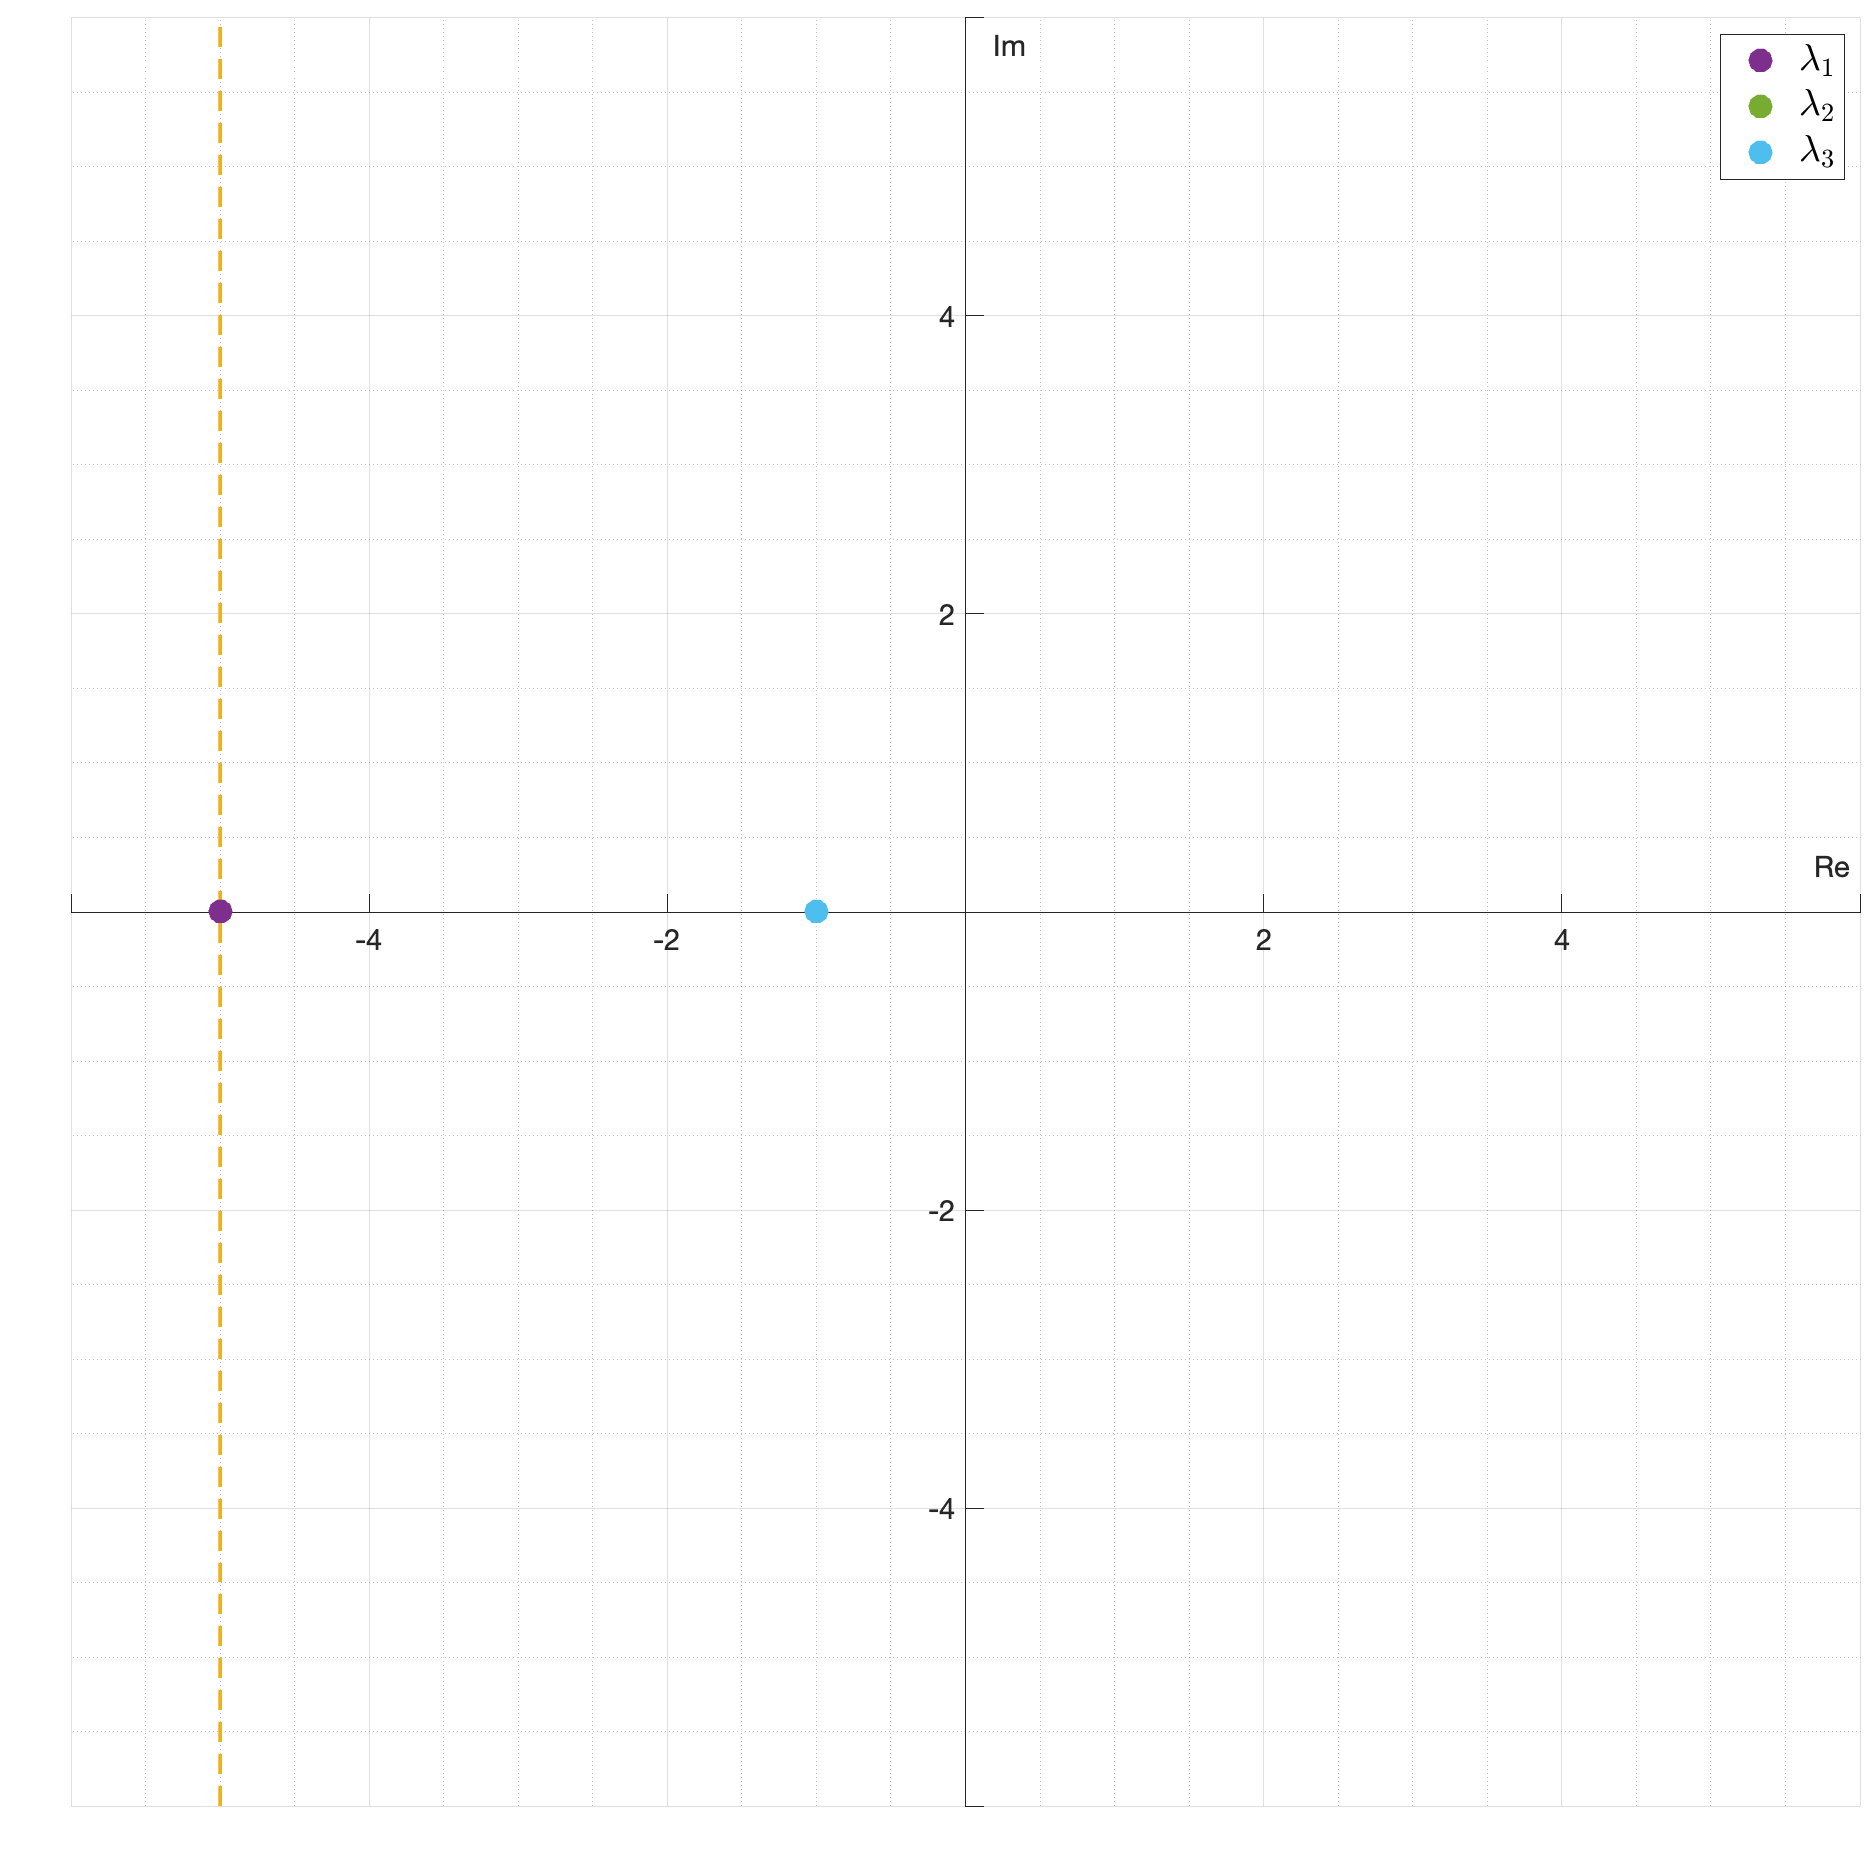
\includegraphics[width=0.8\textwidth]{media/plots/task2_points5.png}
    \caption{Расположение корней на комплексной плоскости в эксперименте 5}
    \label{fig:task_2_points5}
\end{figure}

\begin{figure}
    \centering
    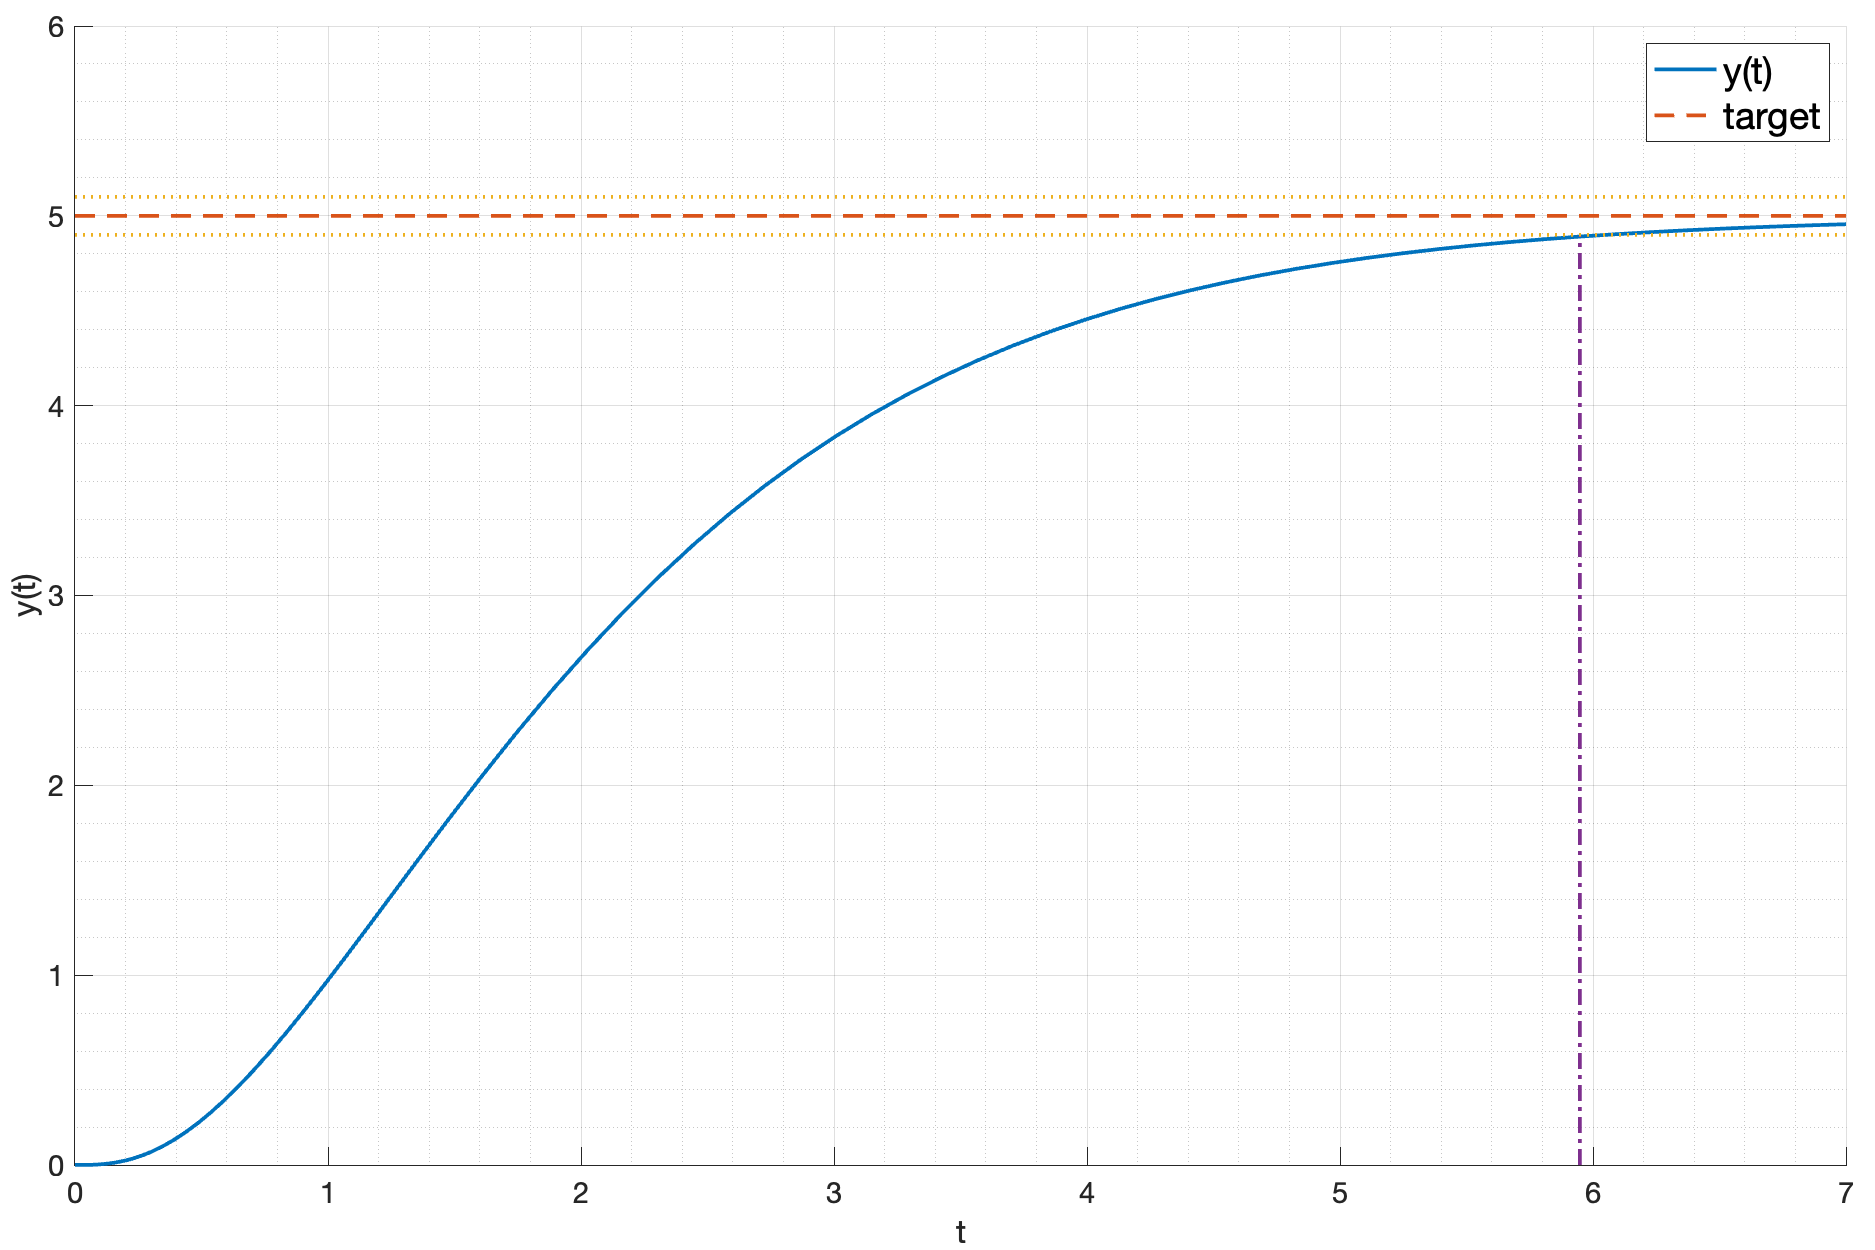
\includegraphics[width=\textwidth]{media/plots/task2_case5.png}
    \caption{Моделирование системы в эксперименте 5}
    \label{fig:task_2_case5}
\end{figure}

Время переходного процесса увеличилось до 5.94 секунды. Таким образом, 
можно сделать вывод, что время переходного процесса зависит от максимального 
значения действительной части корней характеристического уравнения. 

\subsubsection{Эксперемент 6}
\label{task2_case6}
Теперь добавим к корням, рассмотренным в первом эксперименте, сопряженную мнимую часть. 
Рассмотрим набор $\lambda_1 = -3$, $\lambda_2 = -3 - 5i$, $\lambda_3 = -3 + 5i$.
Расположение корней и результаты моделирования приведены на рисунках
\ref{fig:task_2_points6} и \ref{fig:task_2_case6}.

\begin{figure}
    \centering
    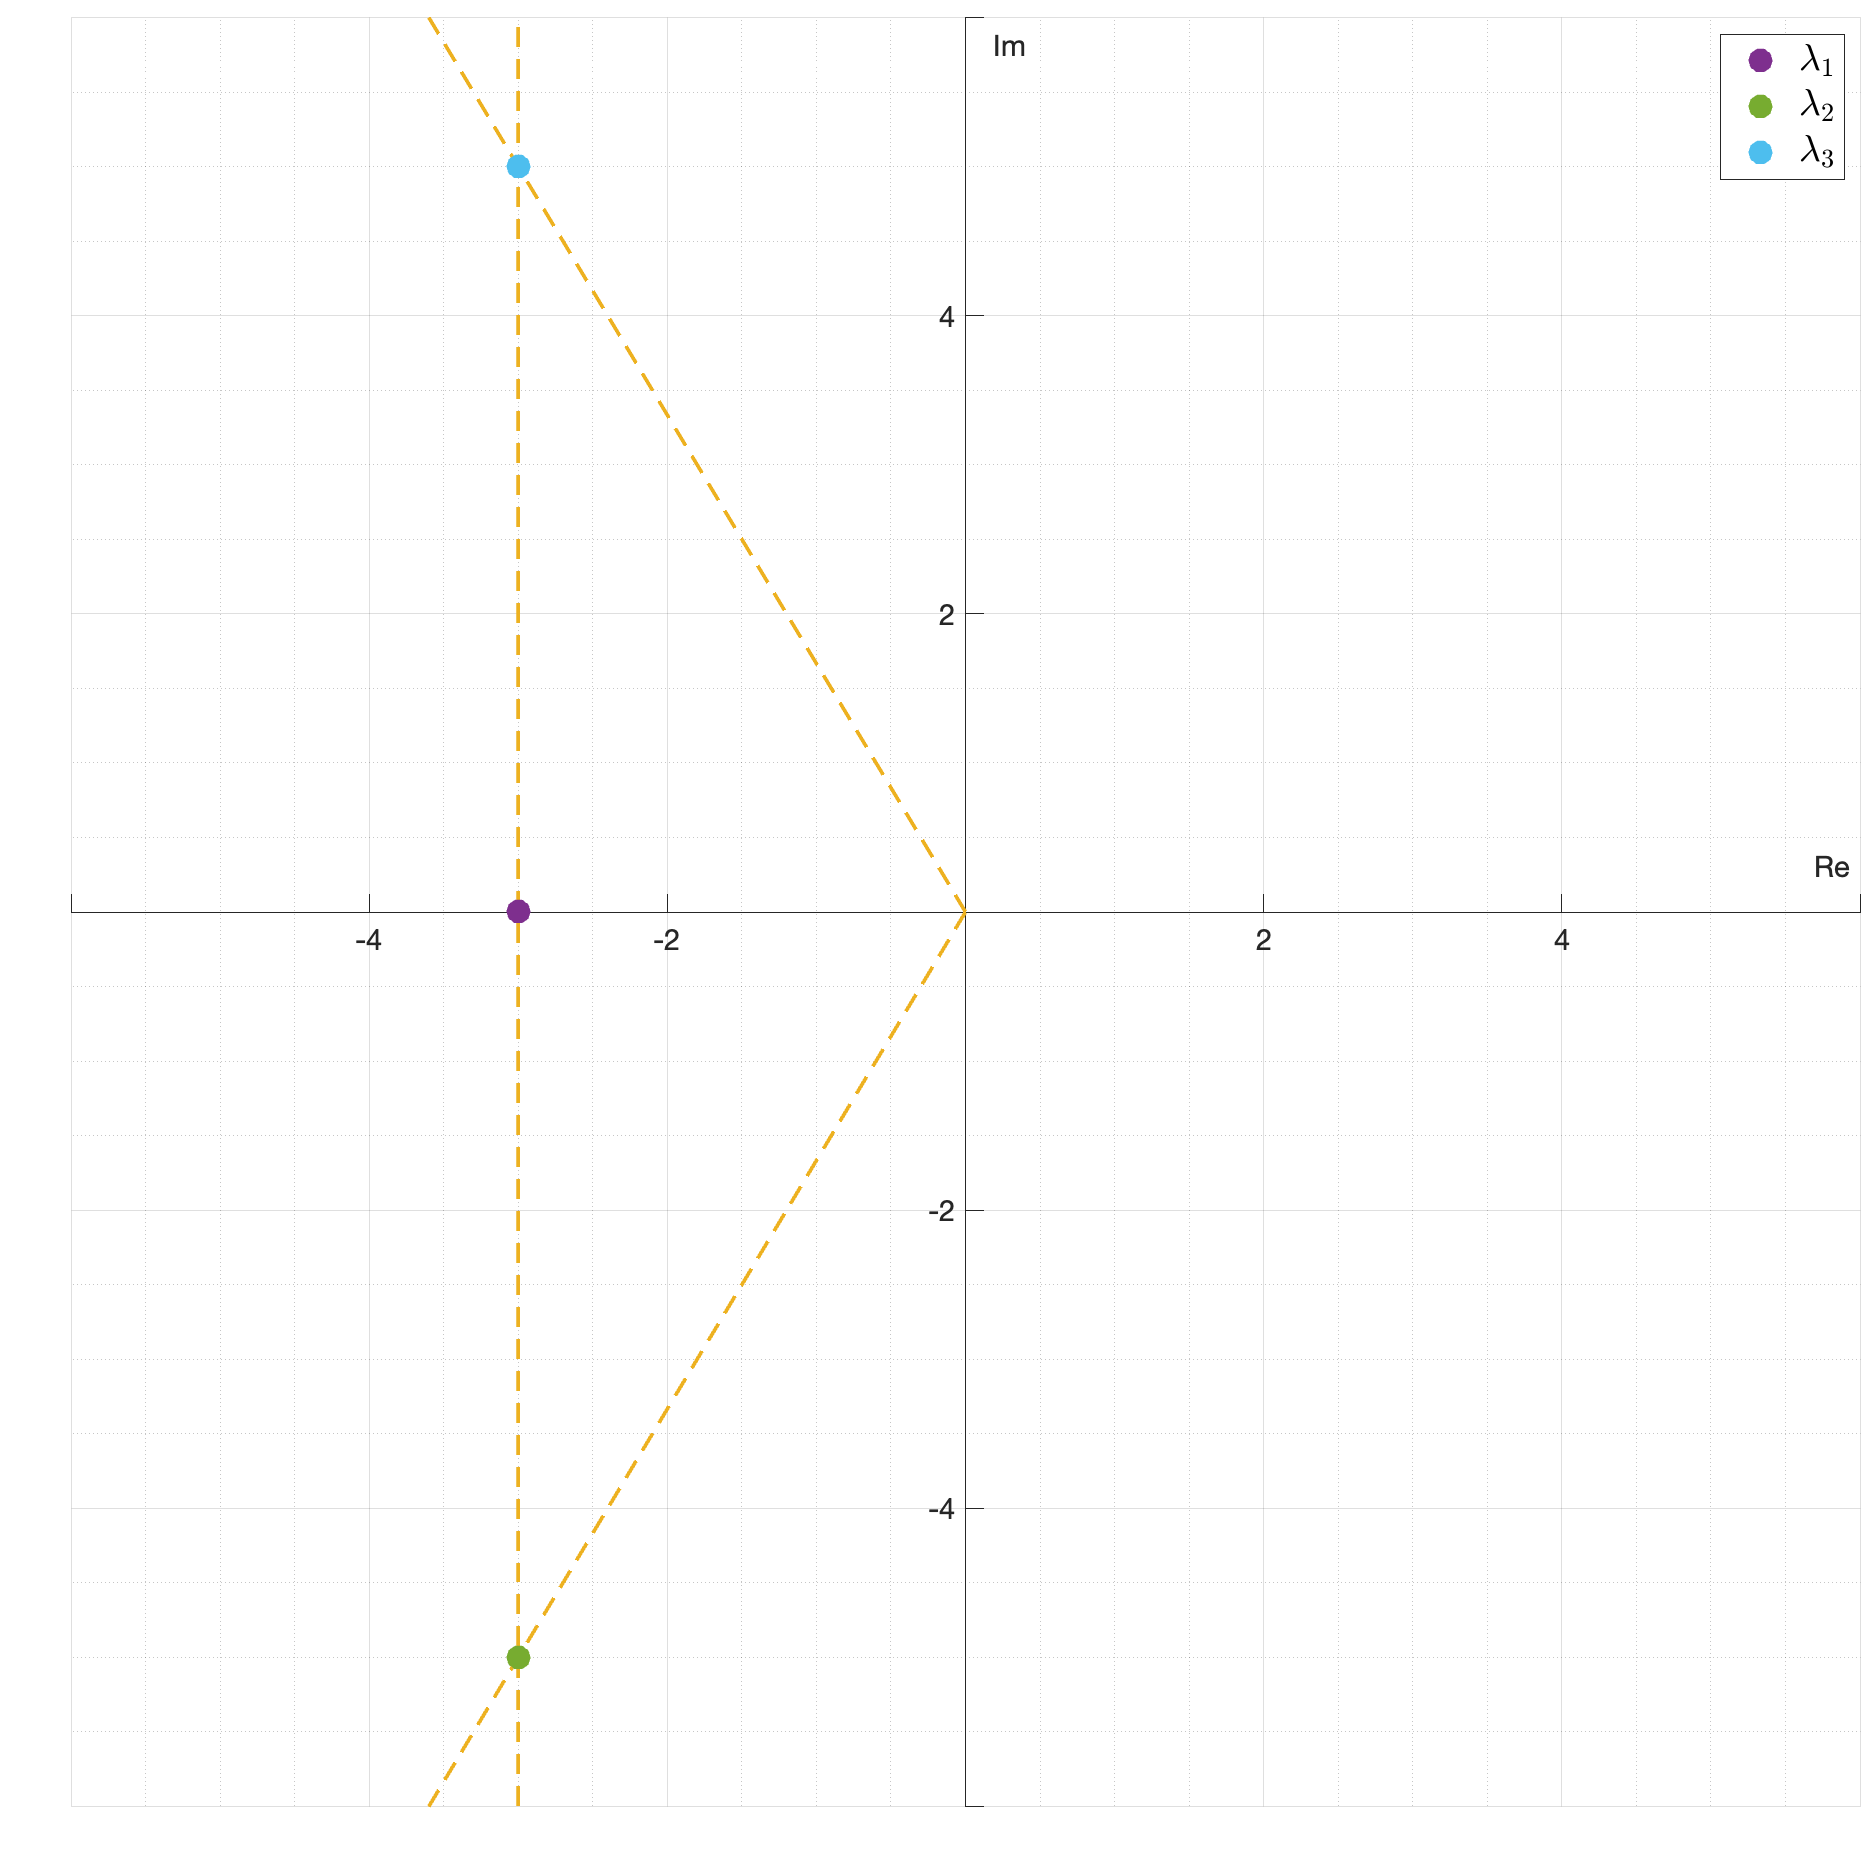
\includegraphics[width=0.8\textwidth]{media/plots/task2_points6.png}
    \caption{Расположение корней на комплексной плоскости в эксперименте 6}
    \label{fig:task_2_points6}
\end{figure}

\begin{figure}
    \centering
    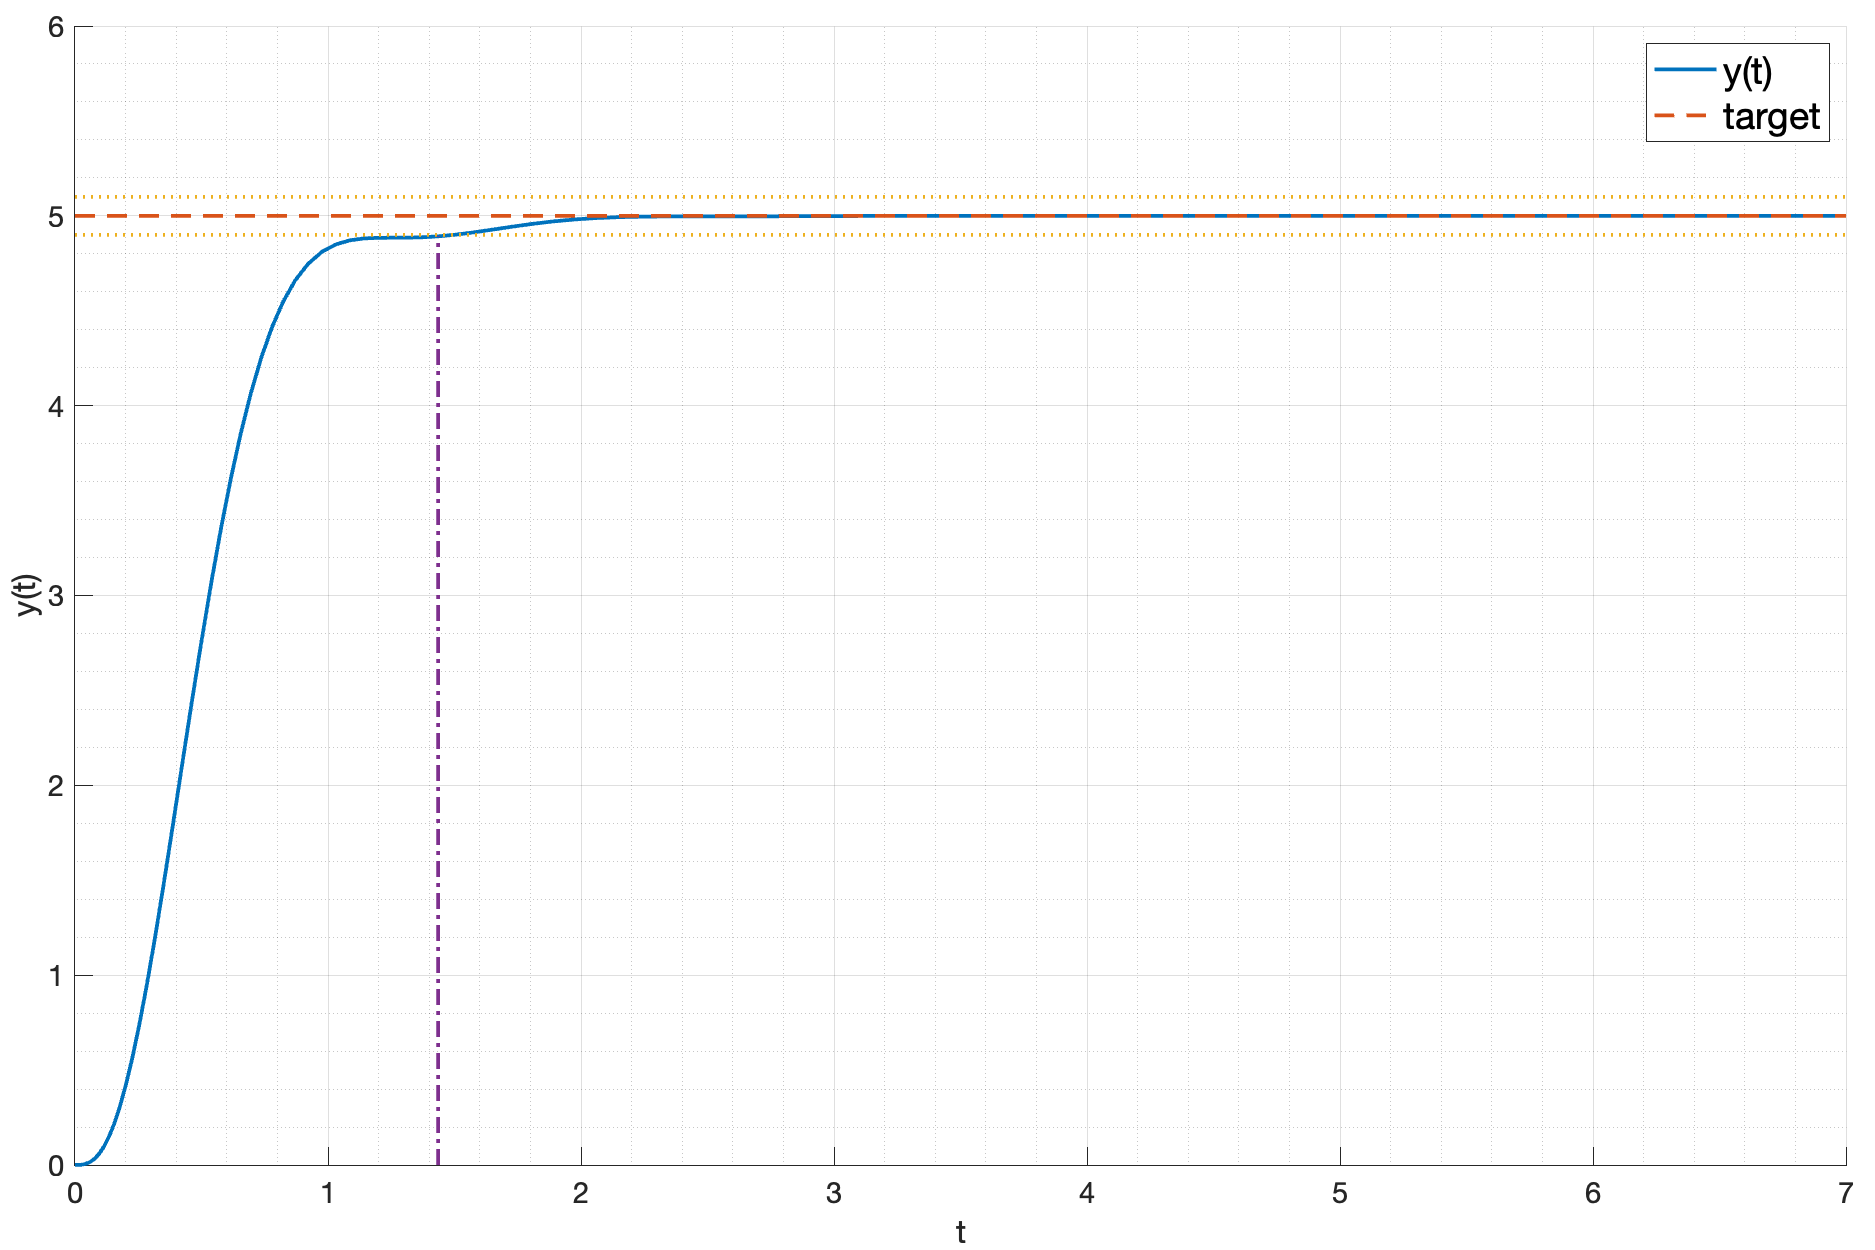
\includegraphics[width=\textwidth]{media/plots/task2_case6.png}
    \caption{Моделирование системы в эксперименте 6}
    \label{fig:task_2_case6}
\end{figure}

Время переходного процесса уменьшилось до 1.43 секунды, перерегулирование все еще отсутствует.

\subsubsection{Эксперемент 7}
\label{task2_case7}
Увеличим по модулю значения мнимых частей корней. Рассмотрим набор 
$\lambda_1 = -3$, $\lambda_2 = -3 - 15i$, $\lambda_3 = -3 + 15i$.
Расположение корней и результаты моделирования приведены на рисунках
\ref{fig:task_2_points7} и \ref{fig:task_2_case7}.

\begin{figure}
    \centering
    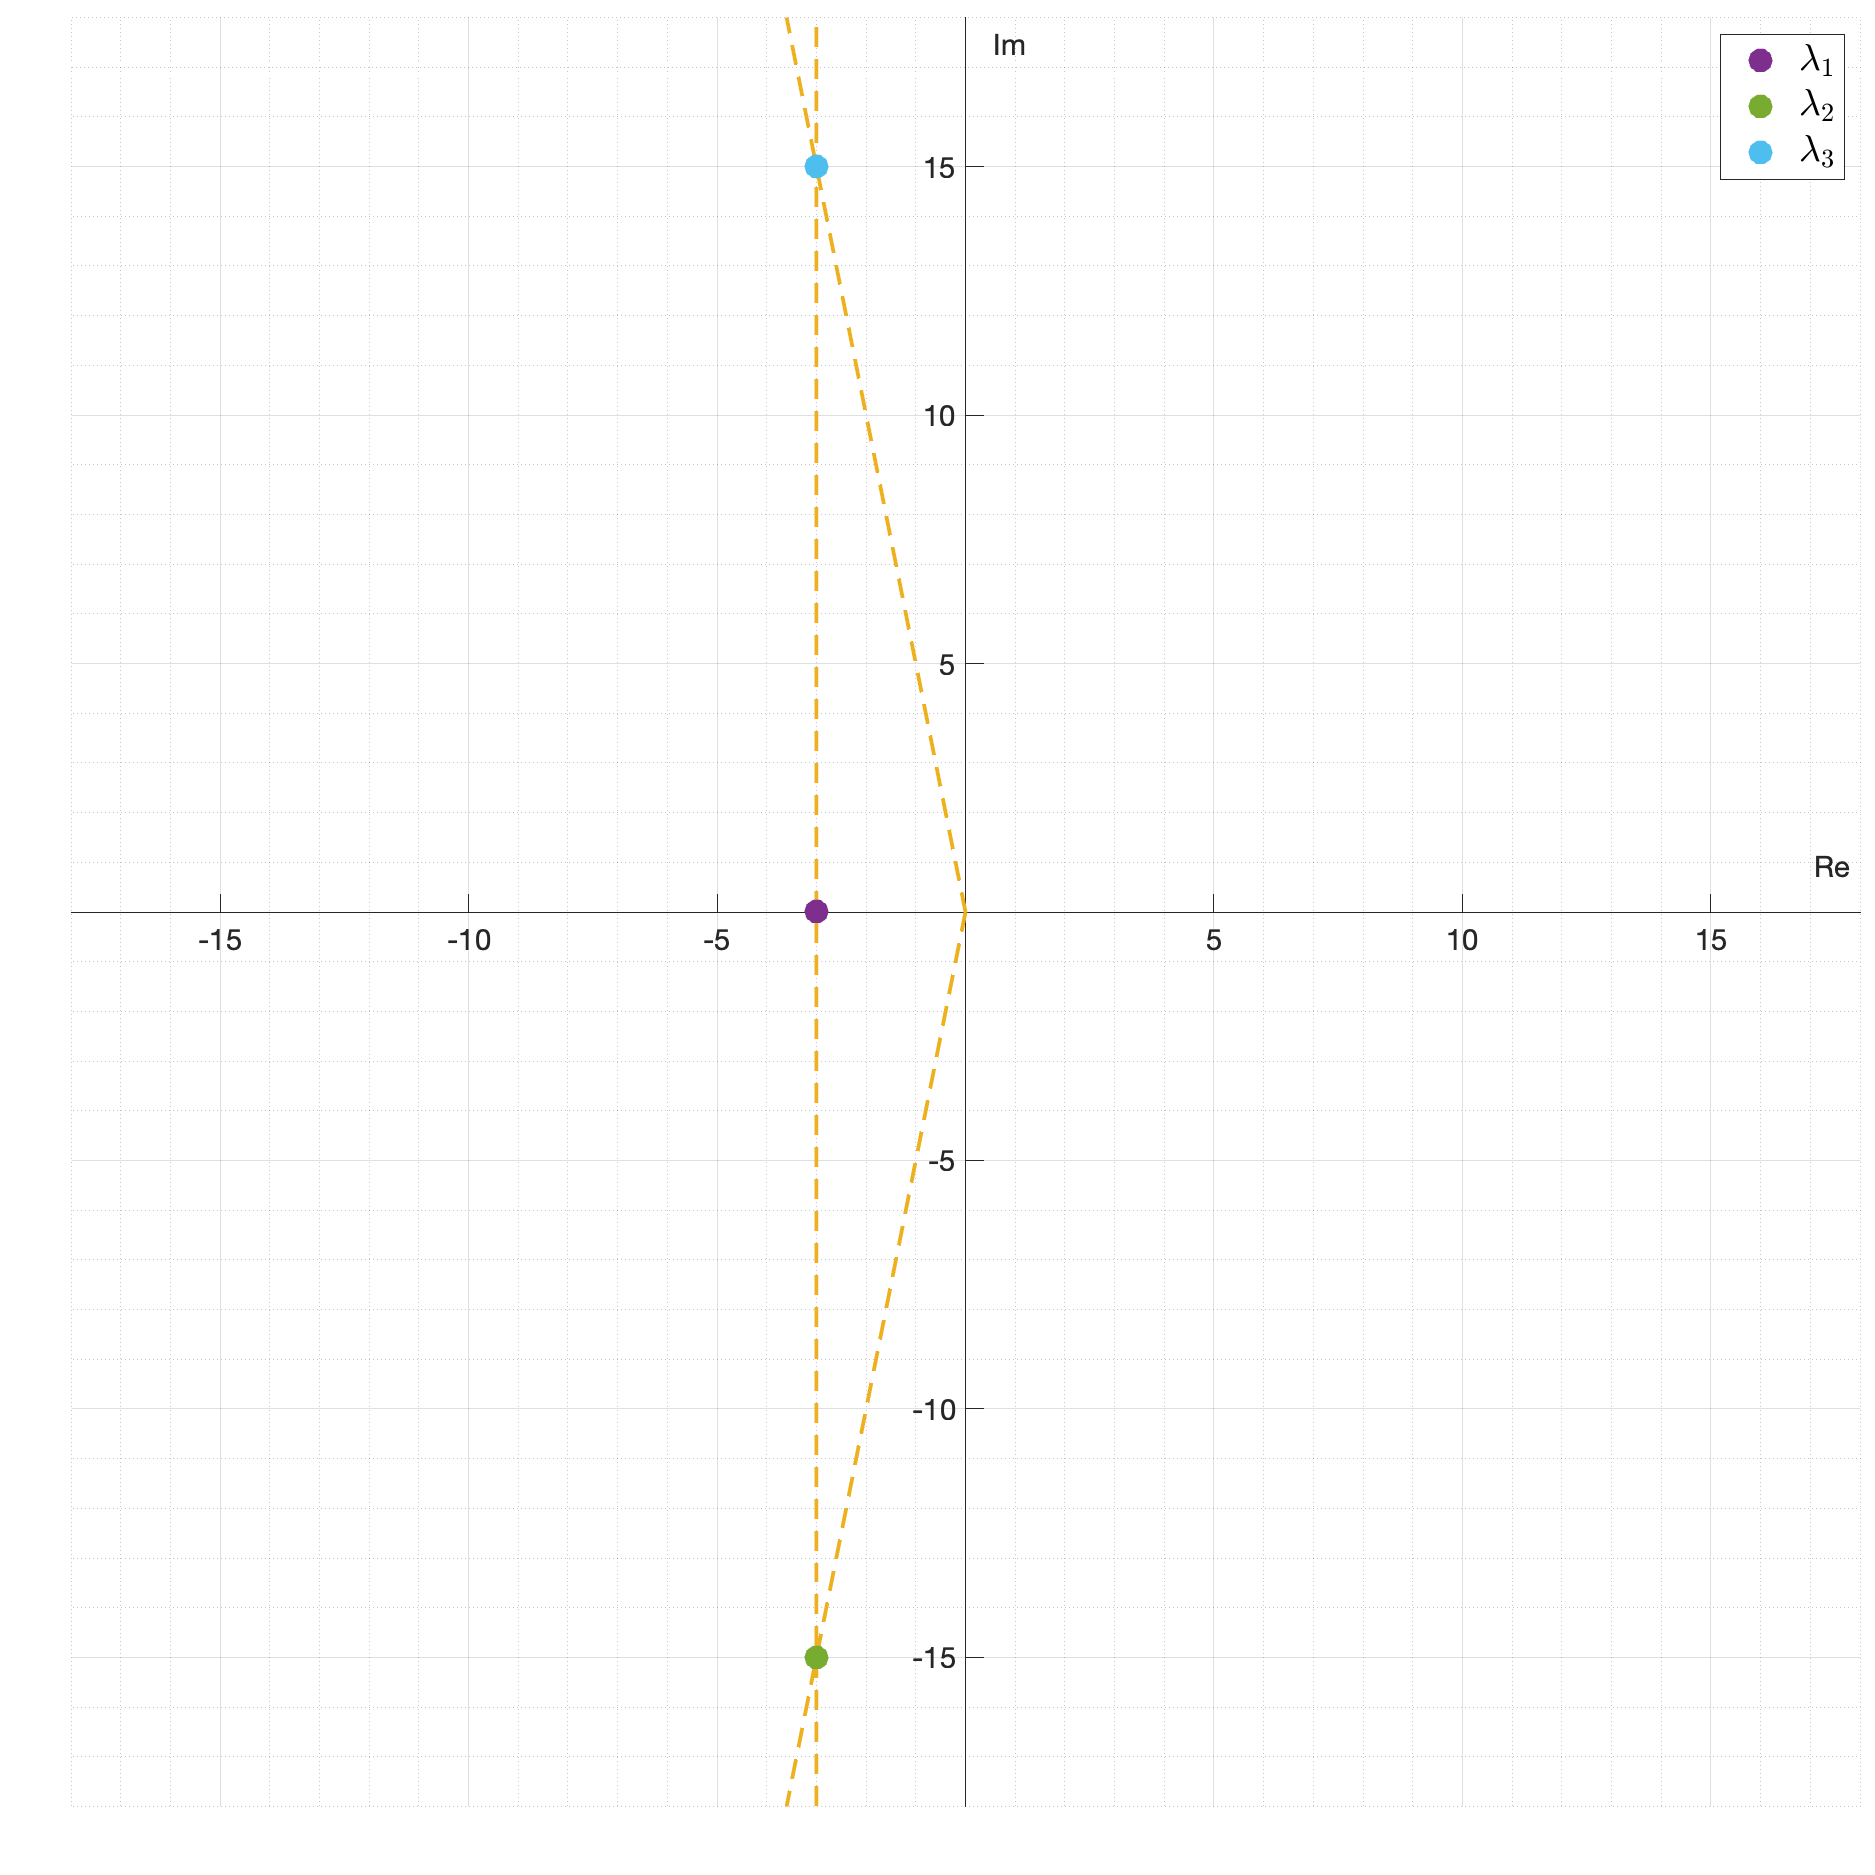
\includegraphics[width=0.8\textwidth]{media/plots/task2_points7.png}
    \caption{Расположение корней на комплексной плоскости в эксперименте 7}
    \label{fig:task_2_points7}
\end{figure}

\begin{figure}
    \centering
    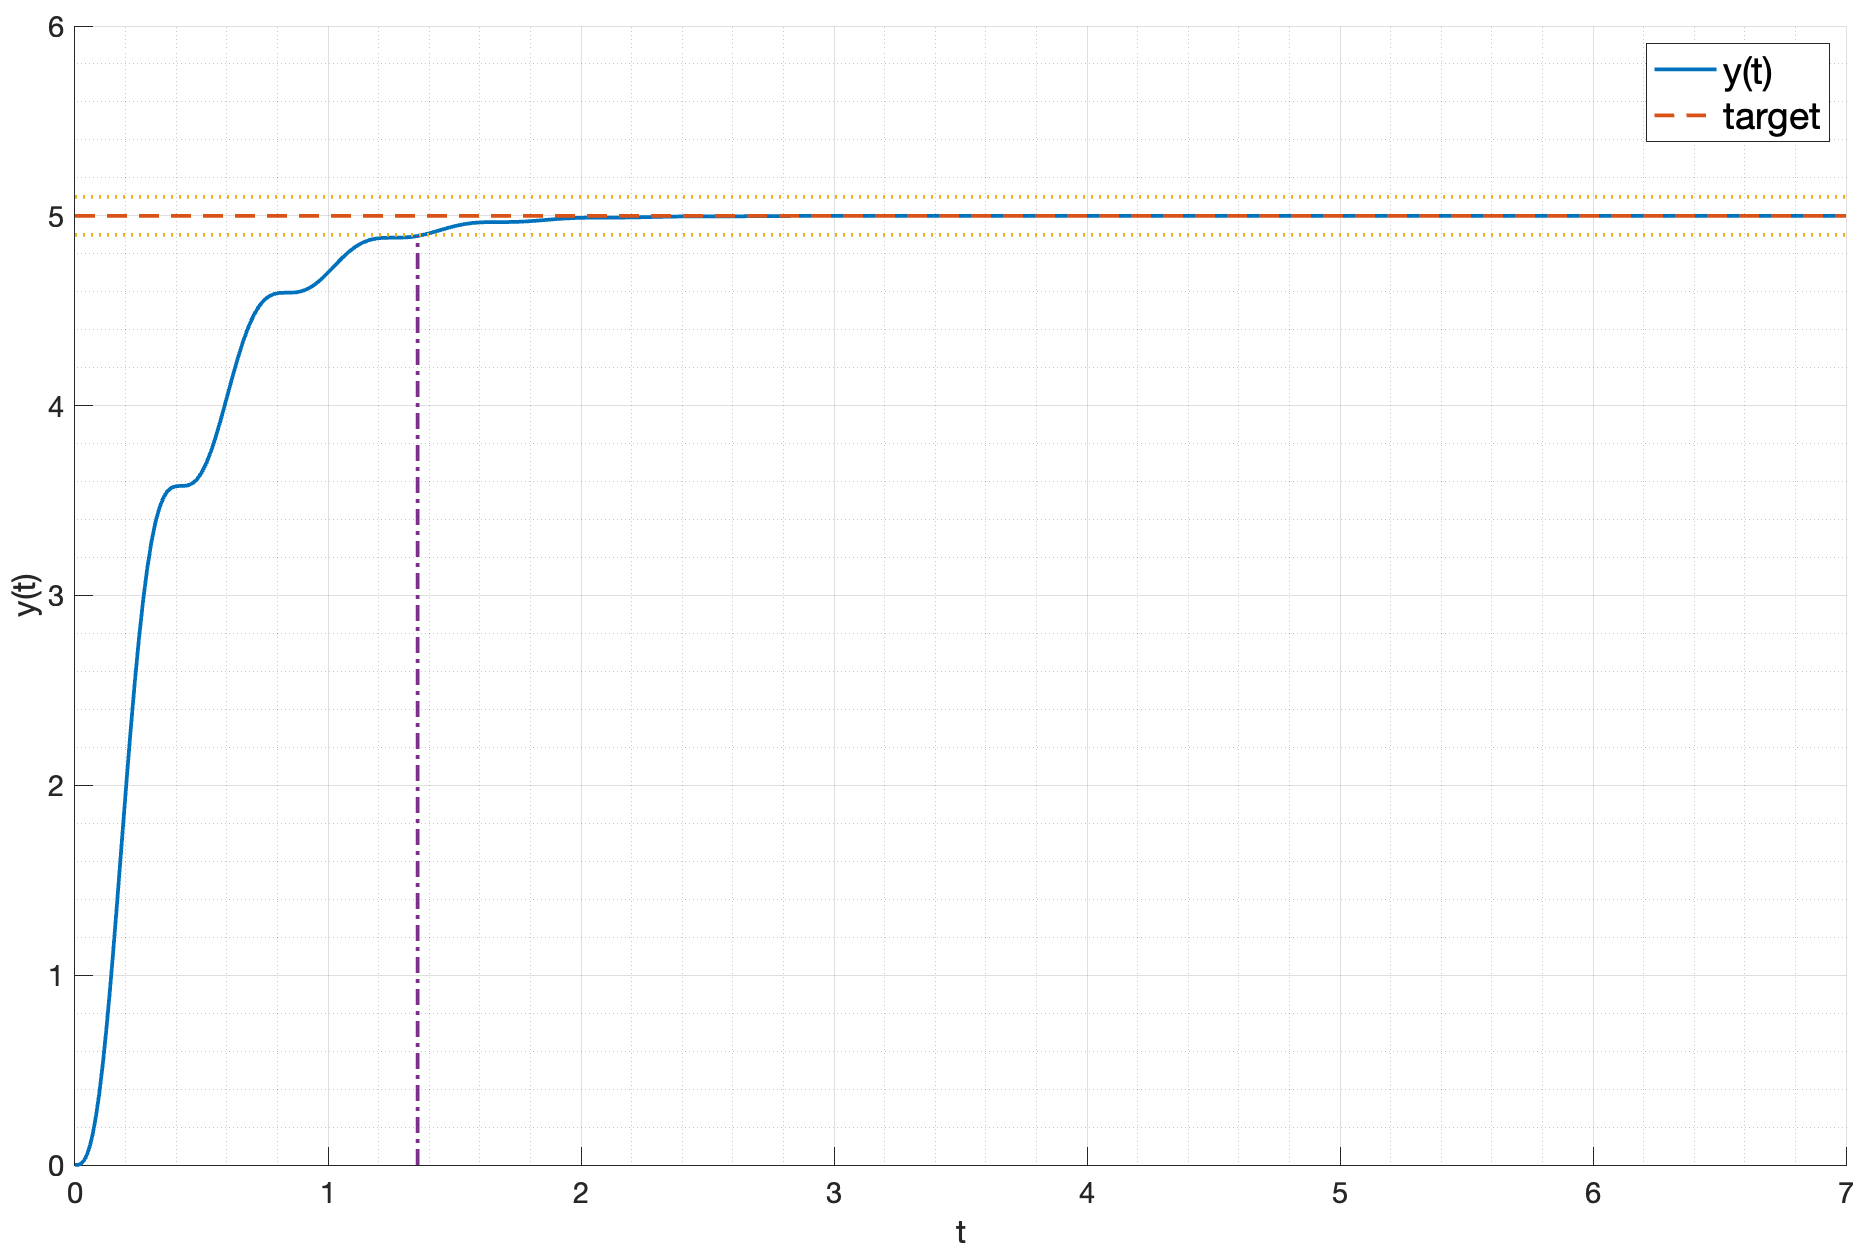
\includegraphics[width=\textwidth]{media/plots/task2_case7.png}
    \caption{Моделирование системы в эксперименте 7}
    \label{fig:task_2_case7}
\end{figure}

Время переходного процесса еще немного уменьшилось и составило 1.35 секунды. При этом 
переходный процесс стал более колебательным, что видно на графике. При этом перерегулирование 
все еще отсутствует.

\subsubsection{Эксперемент 8}
\label{task2_case8}
Уменьшим по модулю значения вещественных частей корней. Рассмотрим набор 
$\lambda_1 = -3$, $\lambda_2 = -1 - 15i$, $\lambda_3 = -1 + 15i$.
Расположение корней и результаты моделирования приведены на рисунках
\ref{fig:task_2_points8} и \ref{fig:task_2_case8}.

\begin{figure}
    \centering
    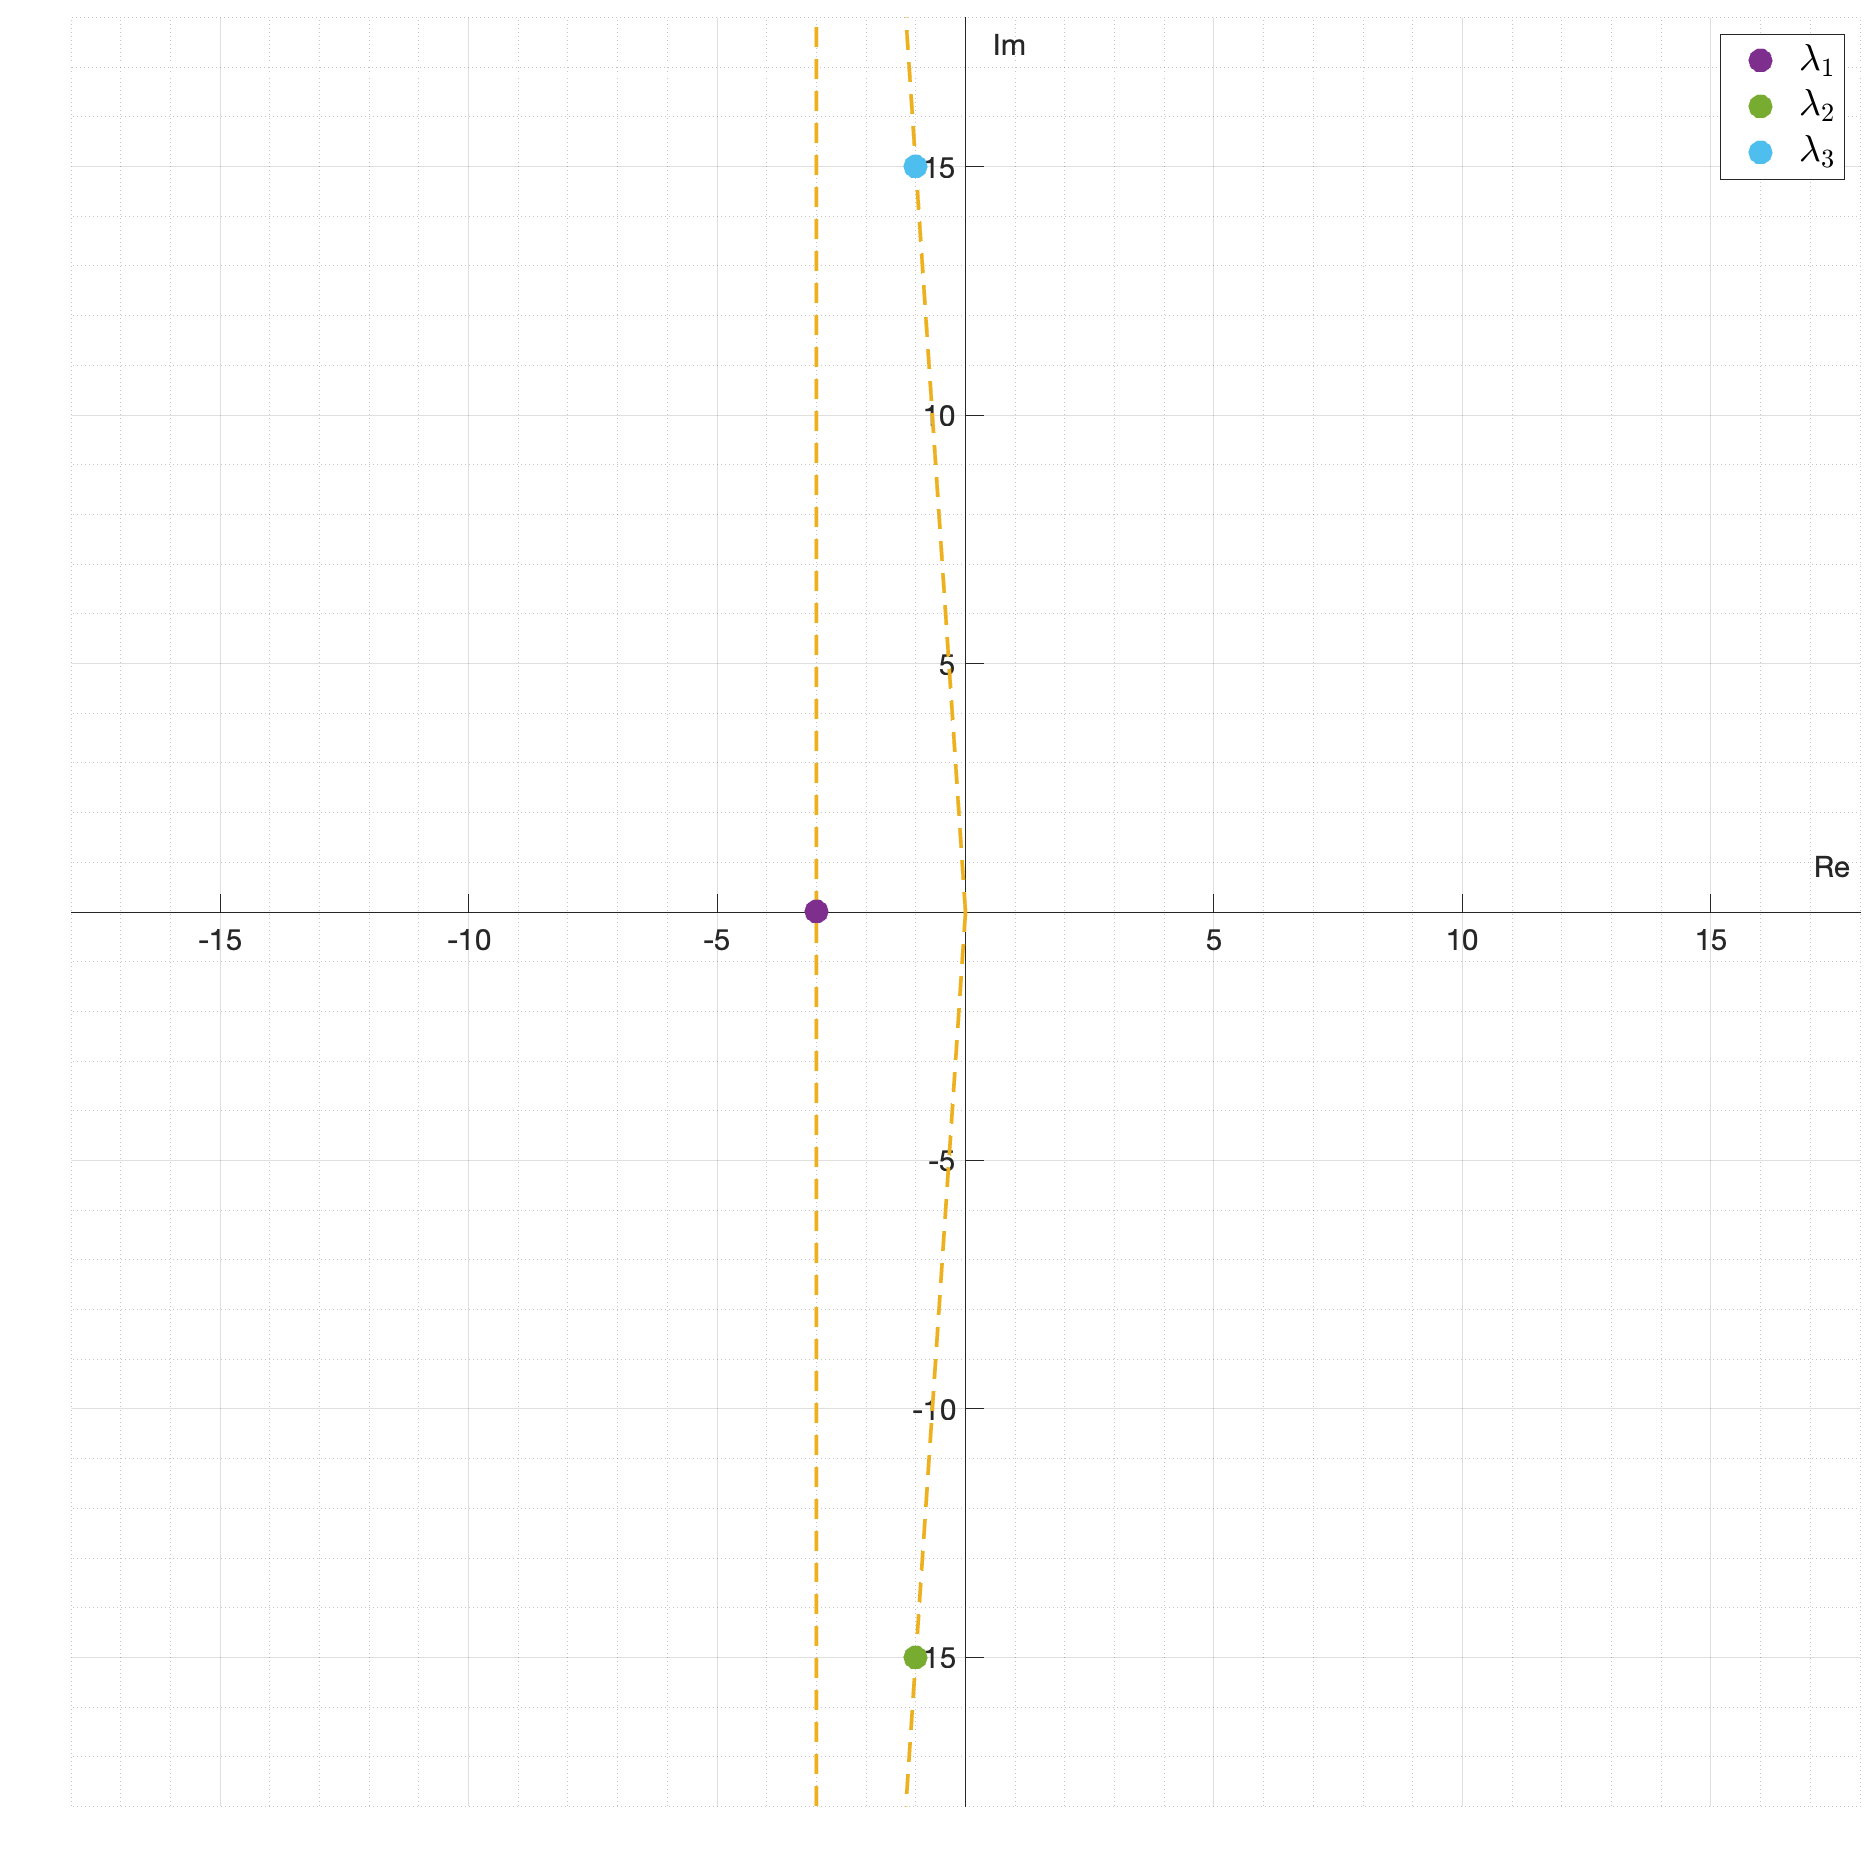
\includegraphics[width=0.8\textwidth]{media/plots/task2_points8.png}
    \caption{Расположение корней на комплексной плоскости в эксперименте 8}
    \label{fig:task_2_points8}
\end{figure}

\begin{figure}
    \centering
    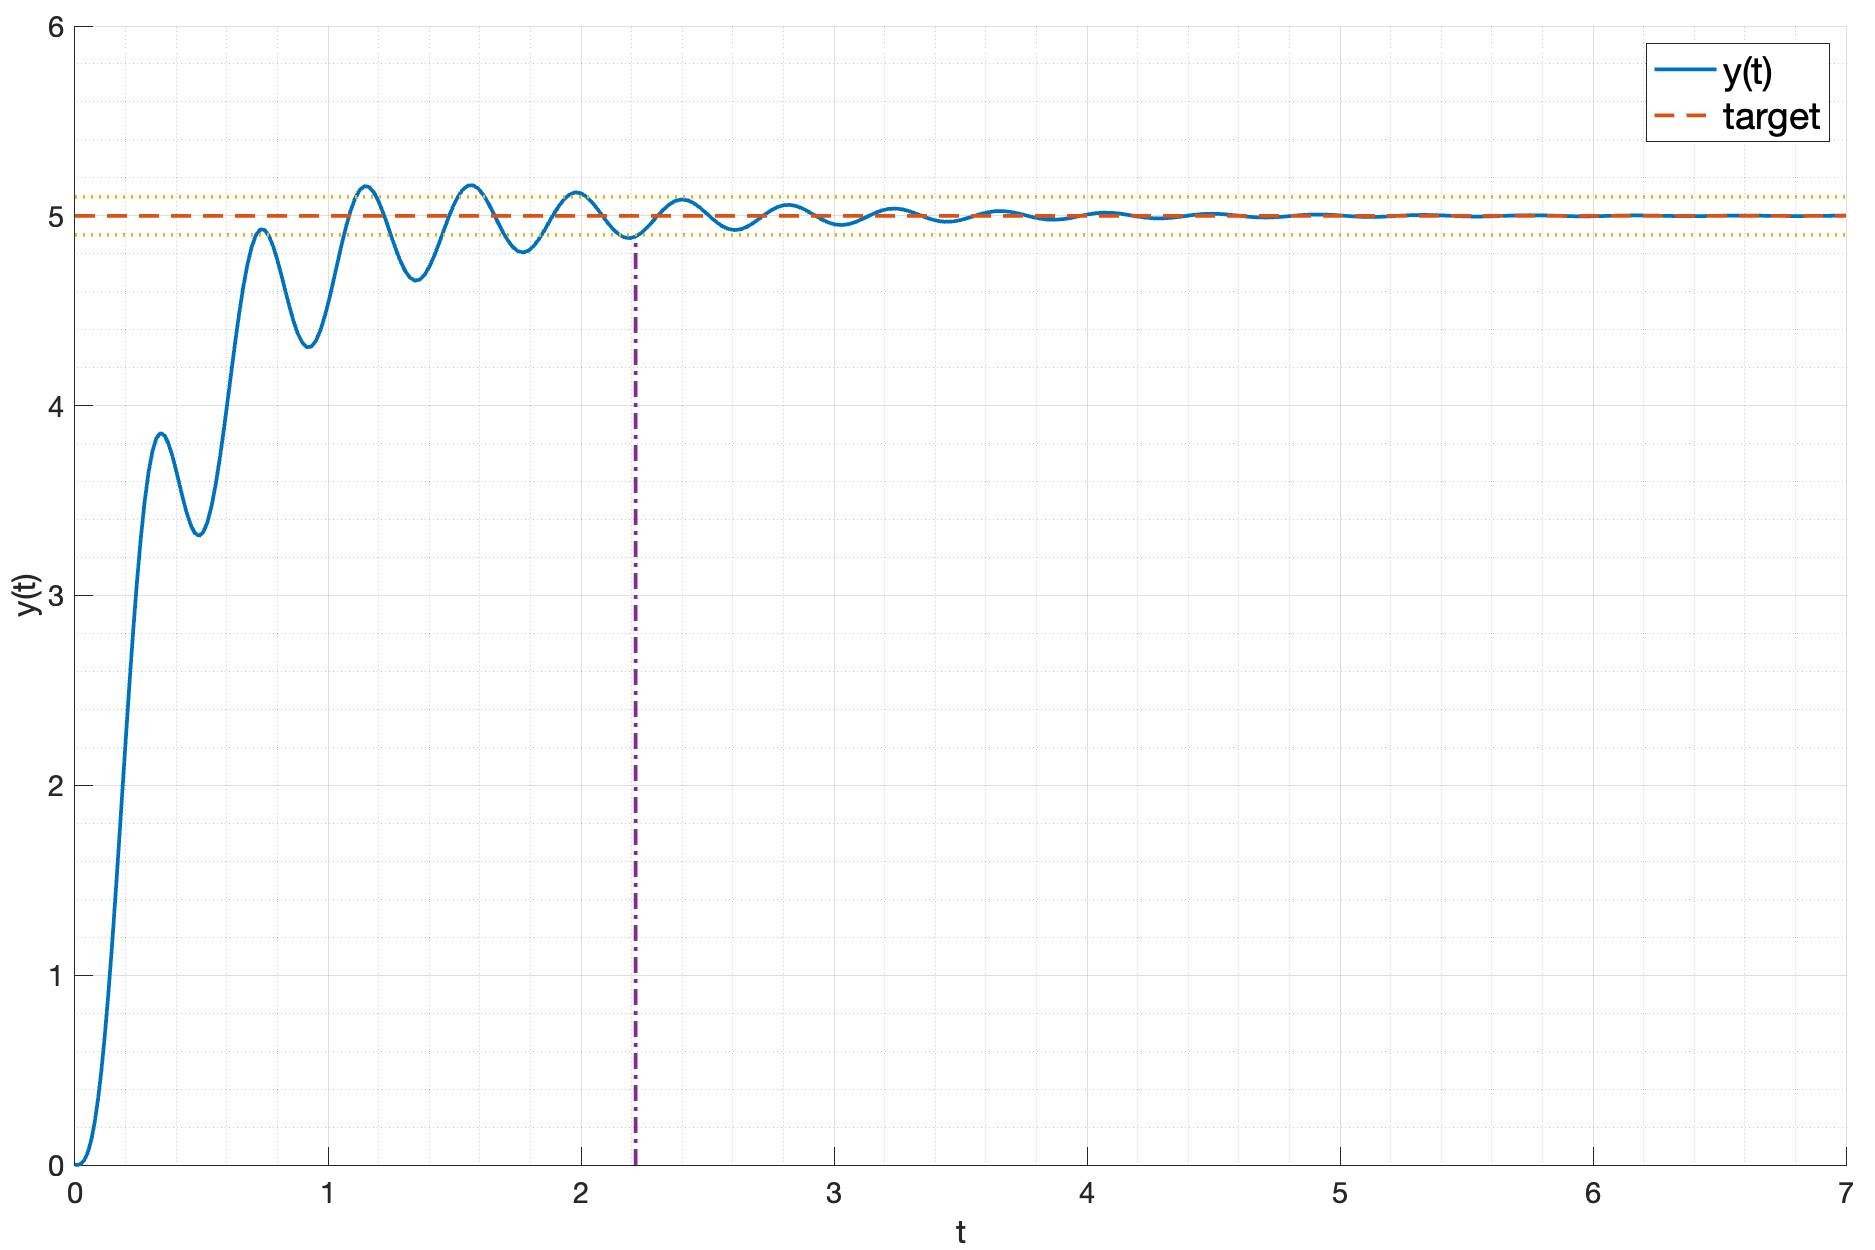
\includegraphics[width=\textwidth]{media/plots/task2_case8.png}
    \caption{Моделирование системы в эксперименте 8}
    \label{fig:task_2_case8}
\end{figure}

Таким образом угол наклона стороны трапеции сильно увеличился, что привело к увеличению
колебательности системы, а вследствие этого и времени переходного процесса до 2.21 секунды. При этом время 
первого вхождения в окрестность установившегося значения уменьшилось.  

Теперь появилось перерегулирование, которое составило 3.2\%. 

\subsubsection{Эксперемент 9}
\label{task2_case9}
Уменьшим значение вещественного корня. Рассмотрим набор
$\lambda_1 = -10$, $\lambda_2 = -1 - 15i$, $\lambda_3 = -1 + 15i$.
Расположение корней и результаты моделирования приведены на рисунках
\ref{fig:task_2_points9} и \ref{fig:task_2_case9}.
\begin{figure}
    \centering
    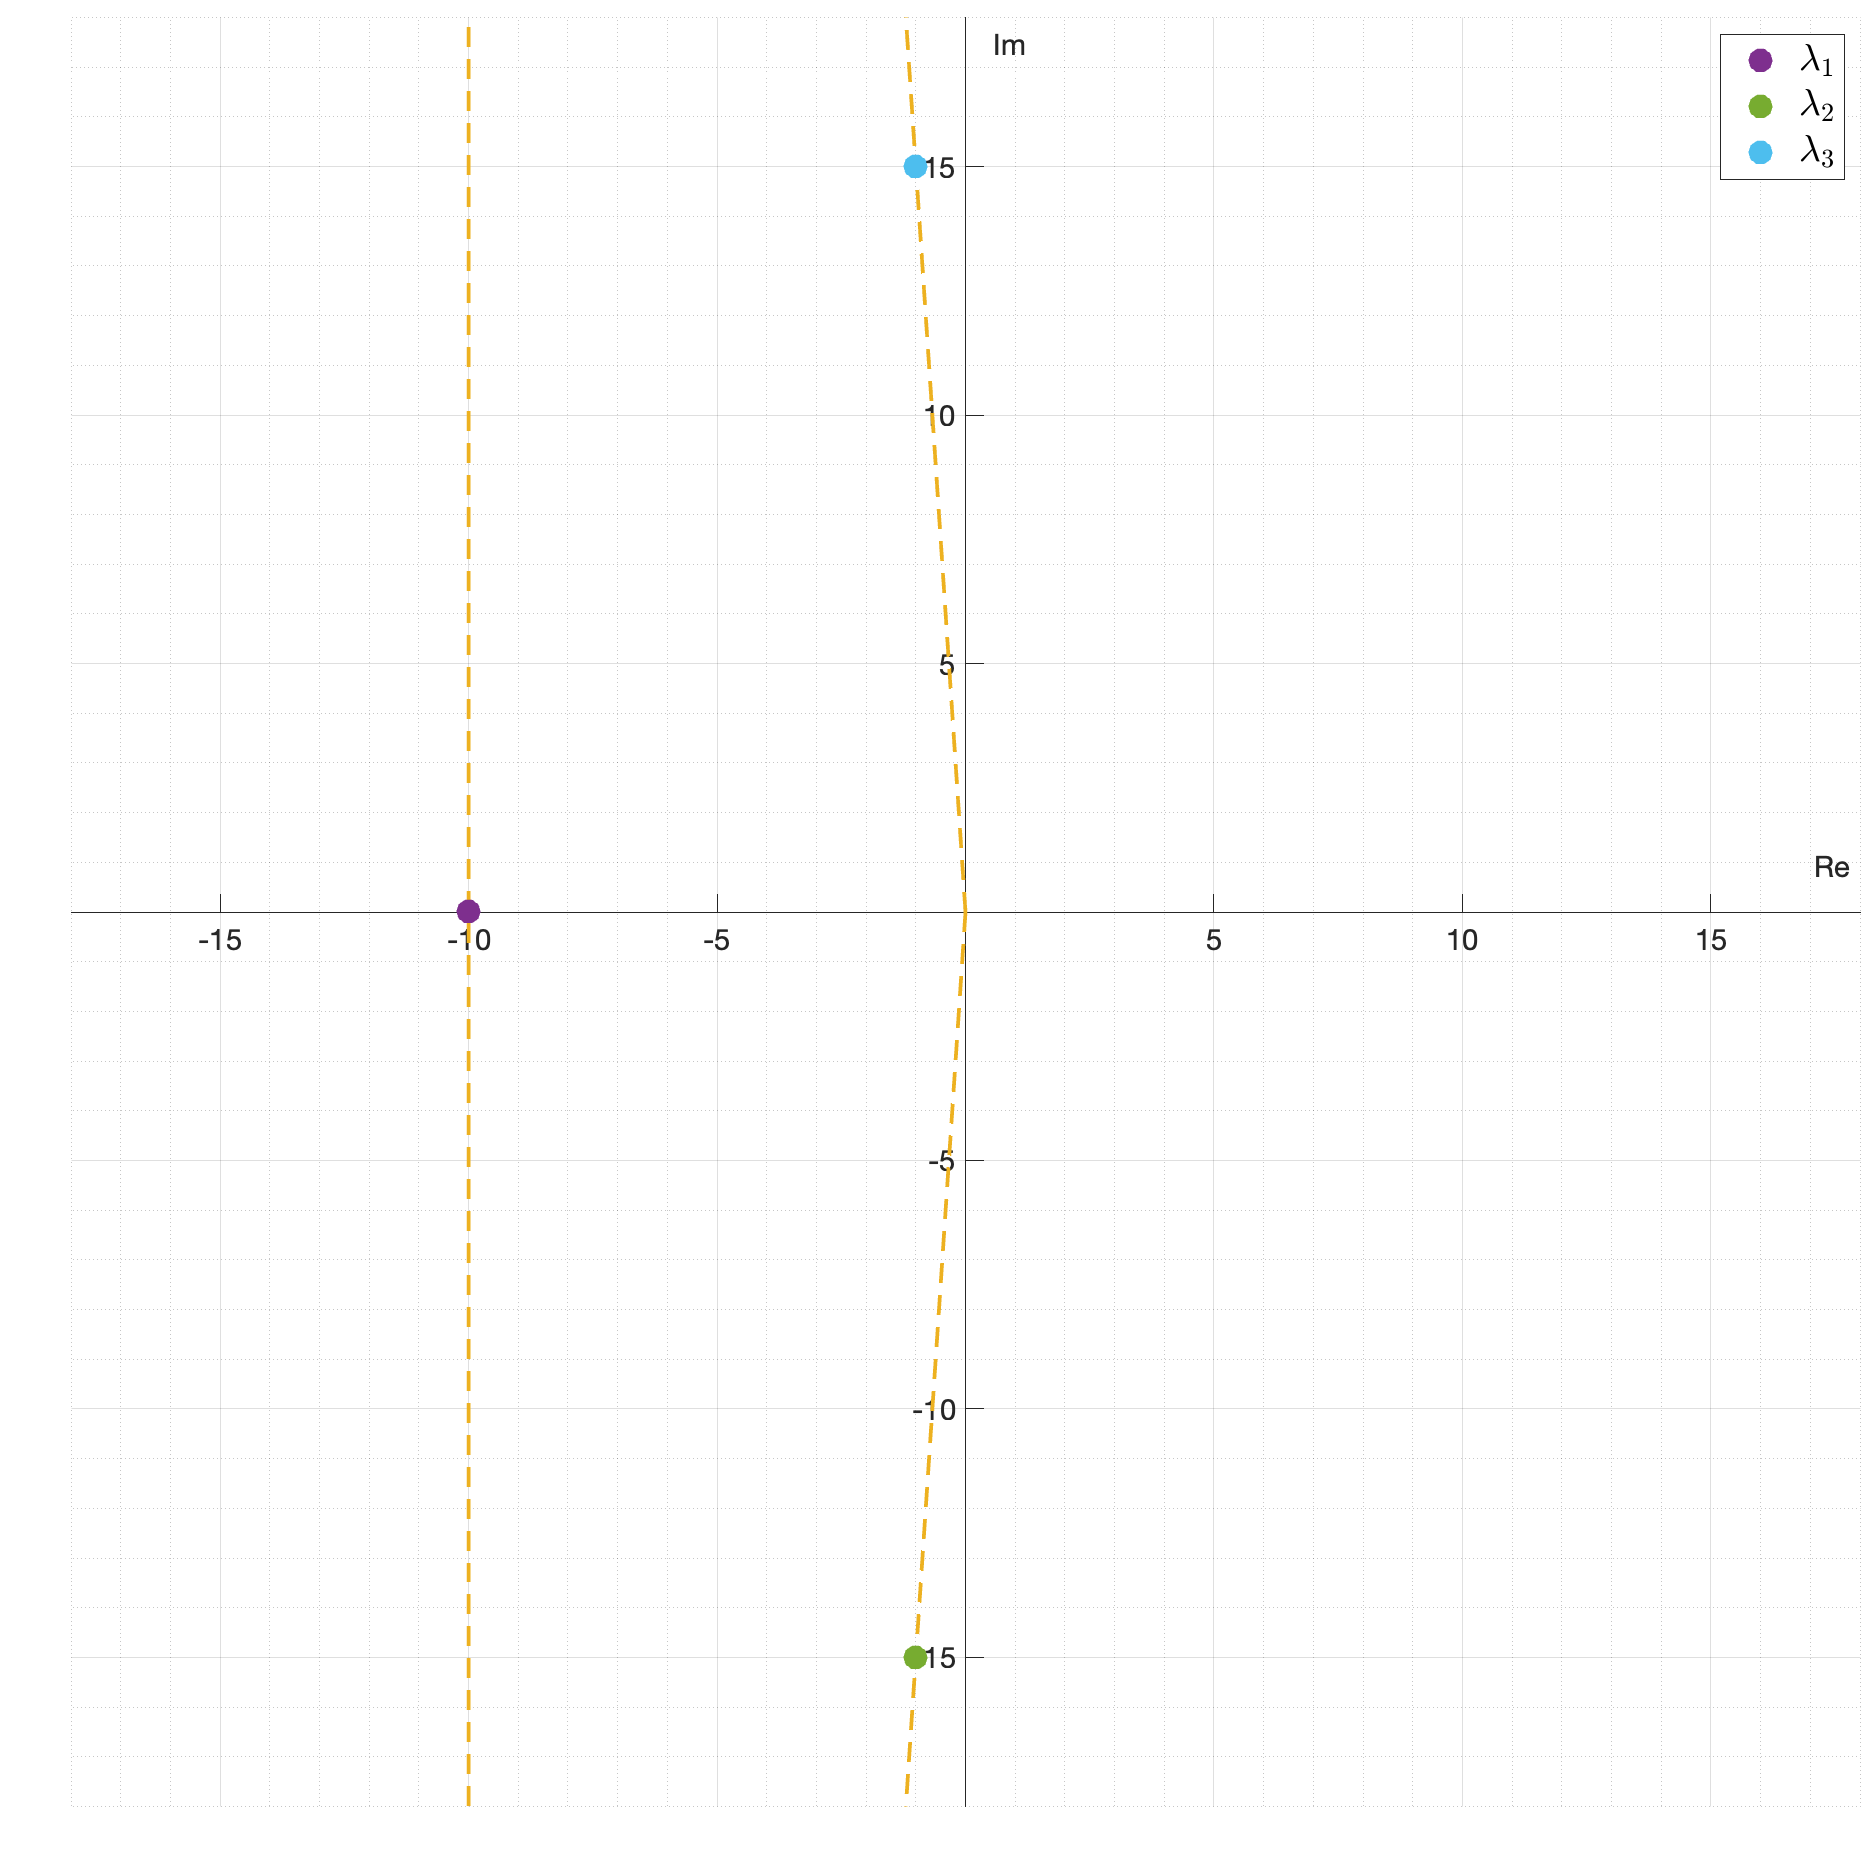
\includegraphics[width=0.8\textwidth]{media/plots/task2_points9.png}
    \caption{Расположение корней на комплексной плоскости в эксперименте 9}
    \label{fig:task_2_points9}
\end{figure}

\begin{figure}
    \centering
    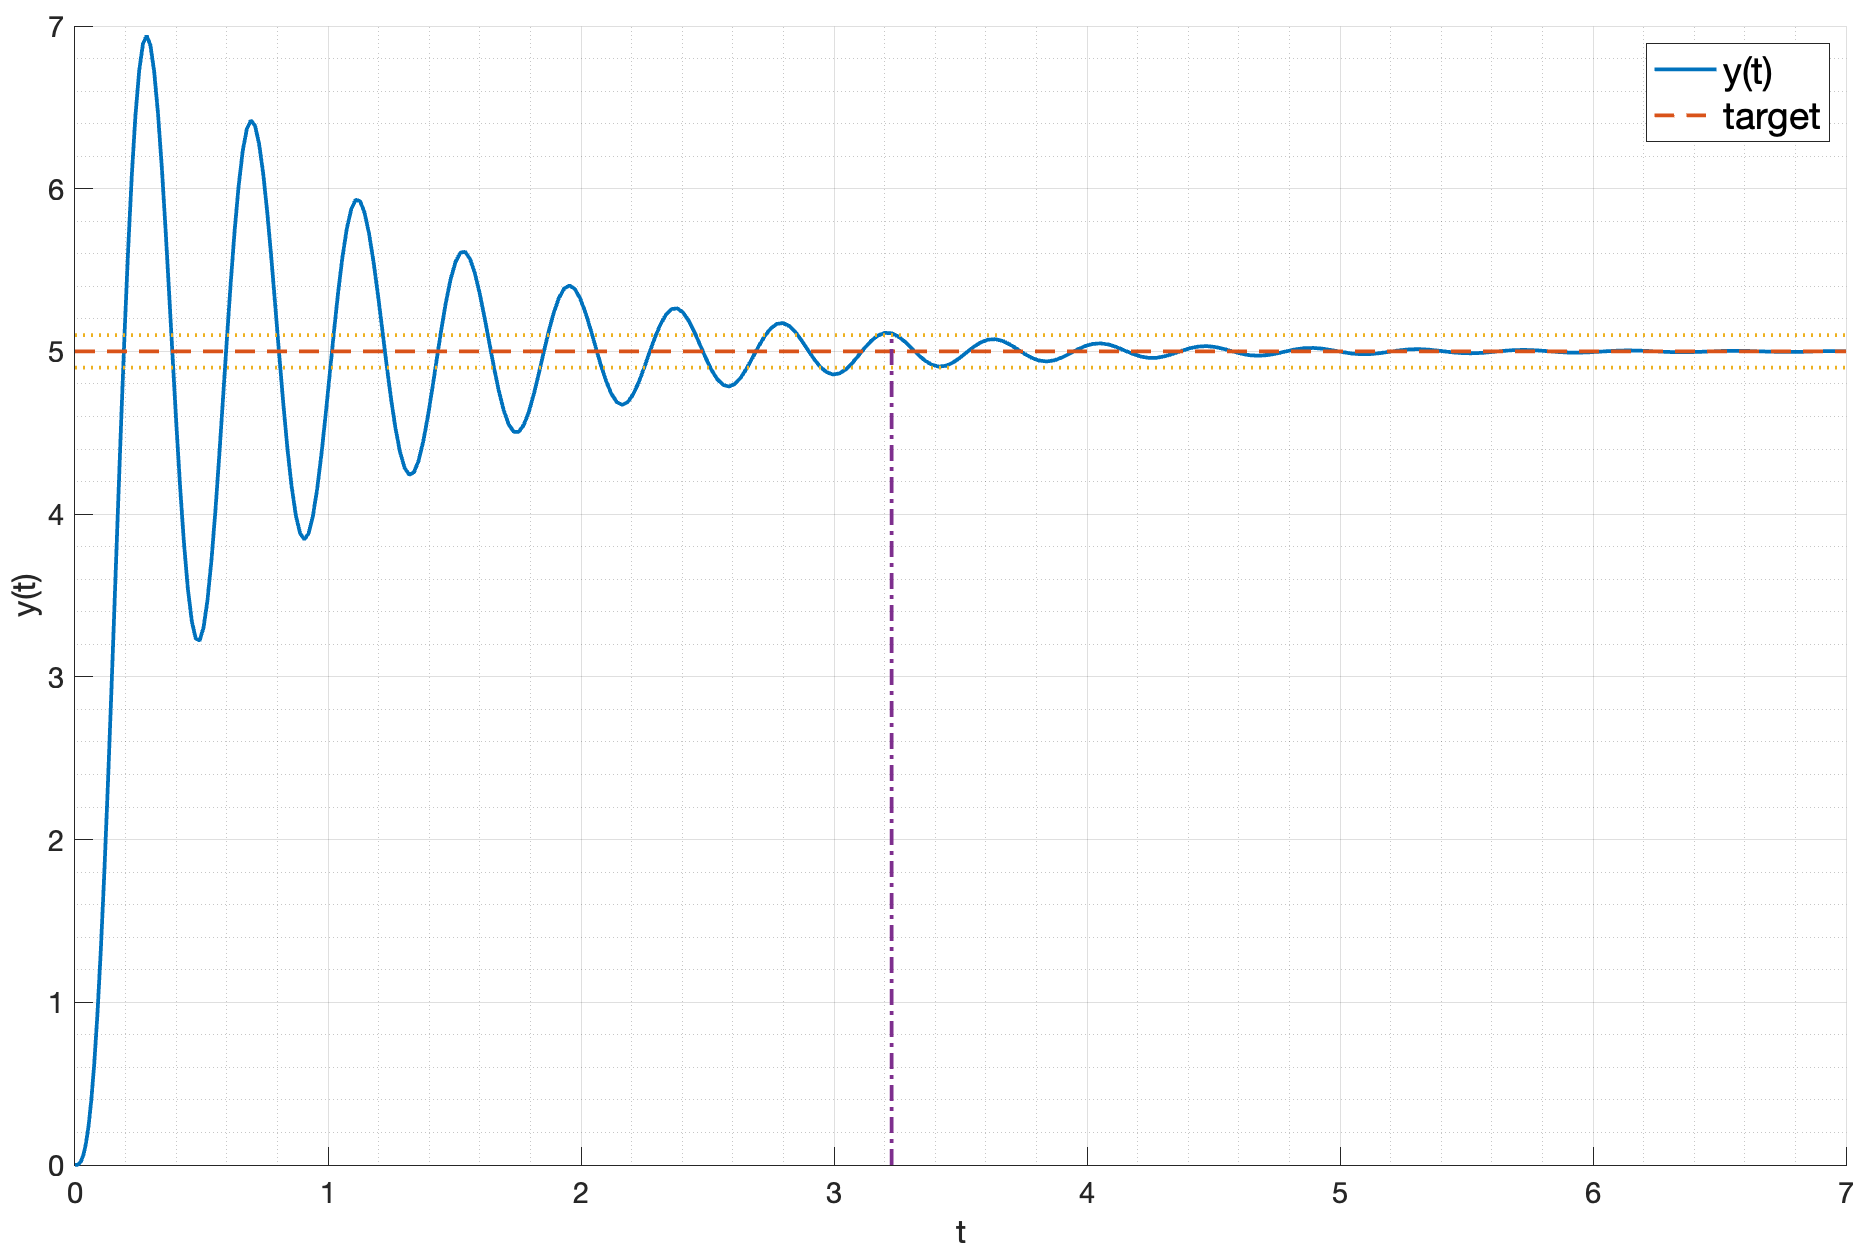
\includegraphics[width=\textwidth]{media/plots/task2_case9.png}
    \caption{Моделирование системы в эксперименте 9}
    \label{fig:task_2_case9}
\end{figure}

Время переходного процесса увеличилось еще сильнее вследствие увеличения колебательности системы.
Теперь оно составляет 3.22 секунды. Перерегулирование увеличилось до 38\%.

\subsubsection{Эксперемент 10}
\label{task2_case10}
Уменьшим вещественную часть сопряженных корней. Рассмотрим набор
$\lambda_1 = -10$, $\lambda_2 = -5 - 15i$, $\lambda_3 = -5 + 15i$.
Расположение корней и результаты моделирования приведены на рисунках
\ref{fig:task_2_points10} и \ref{fig:task_2_case10}.

\begin{figure}
    \centering
    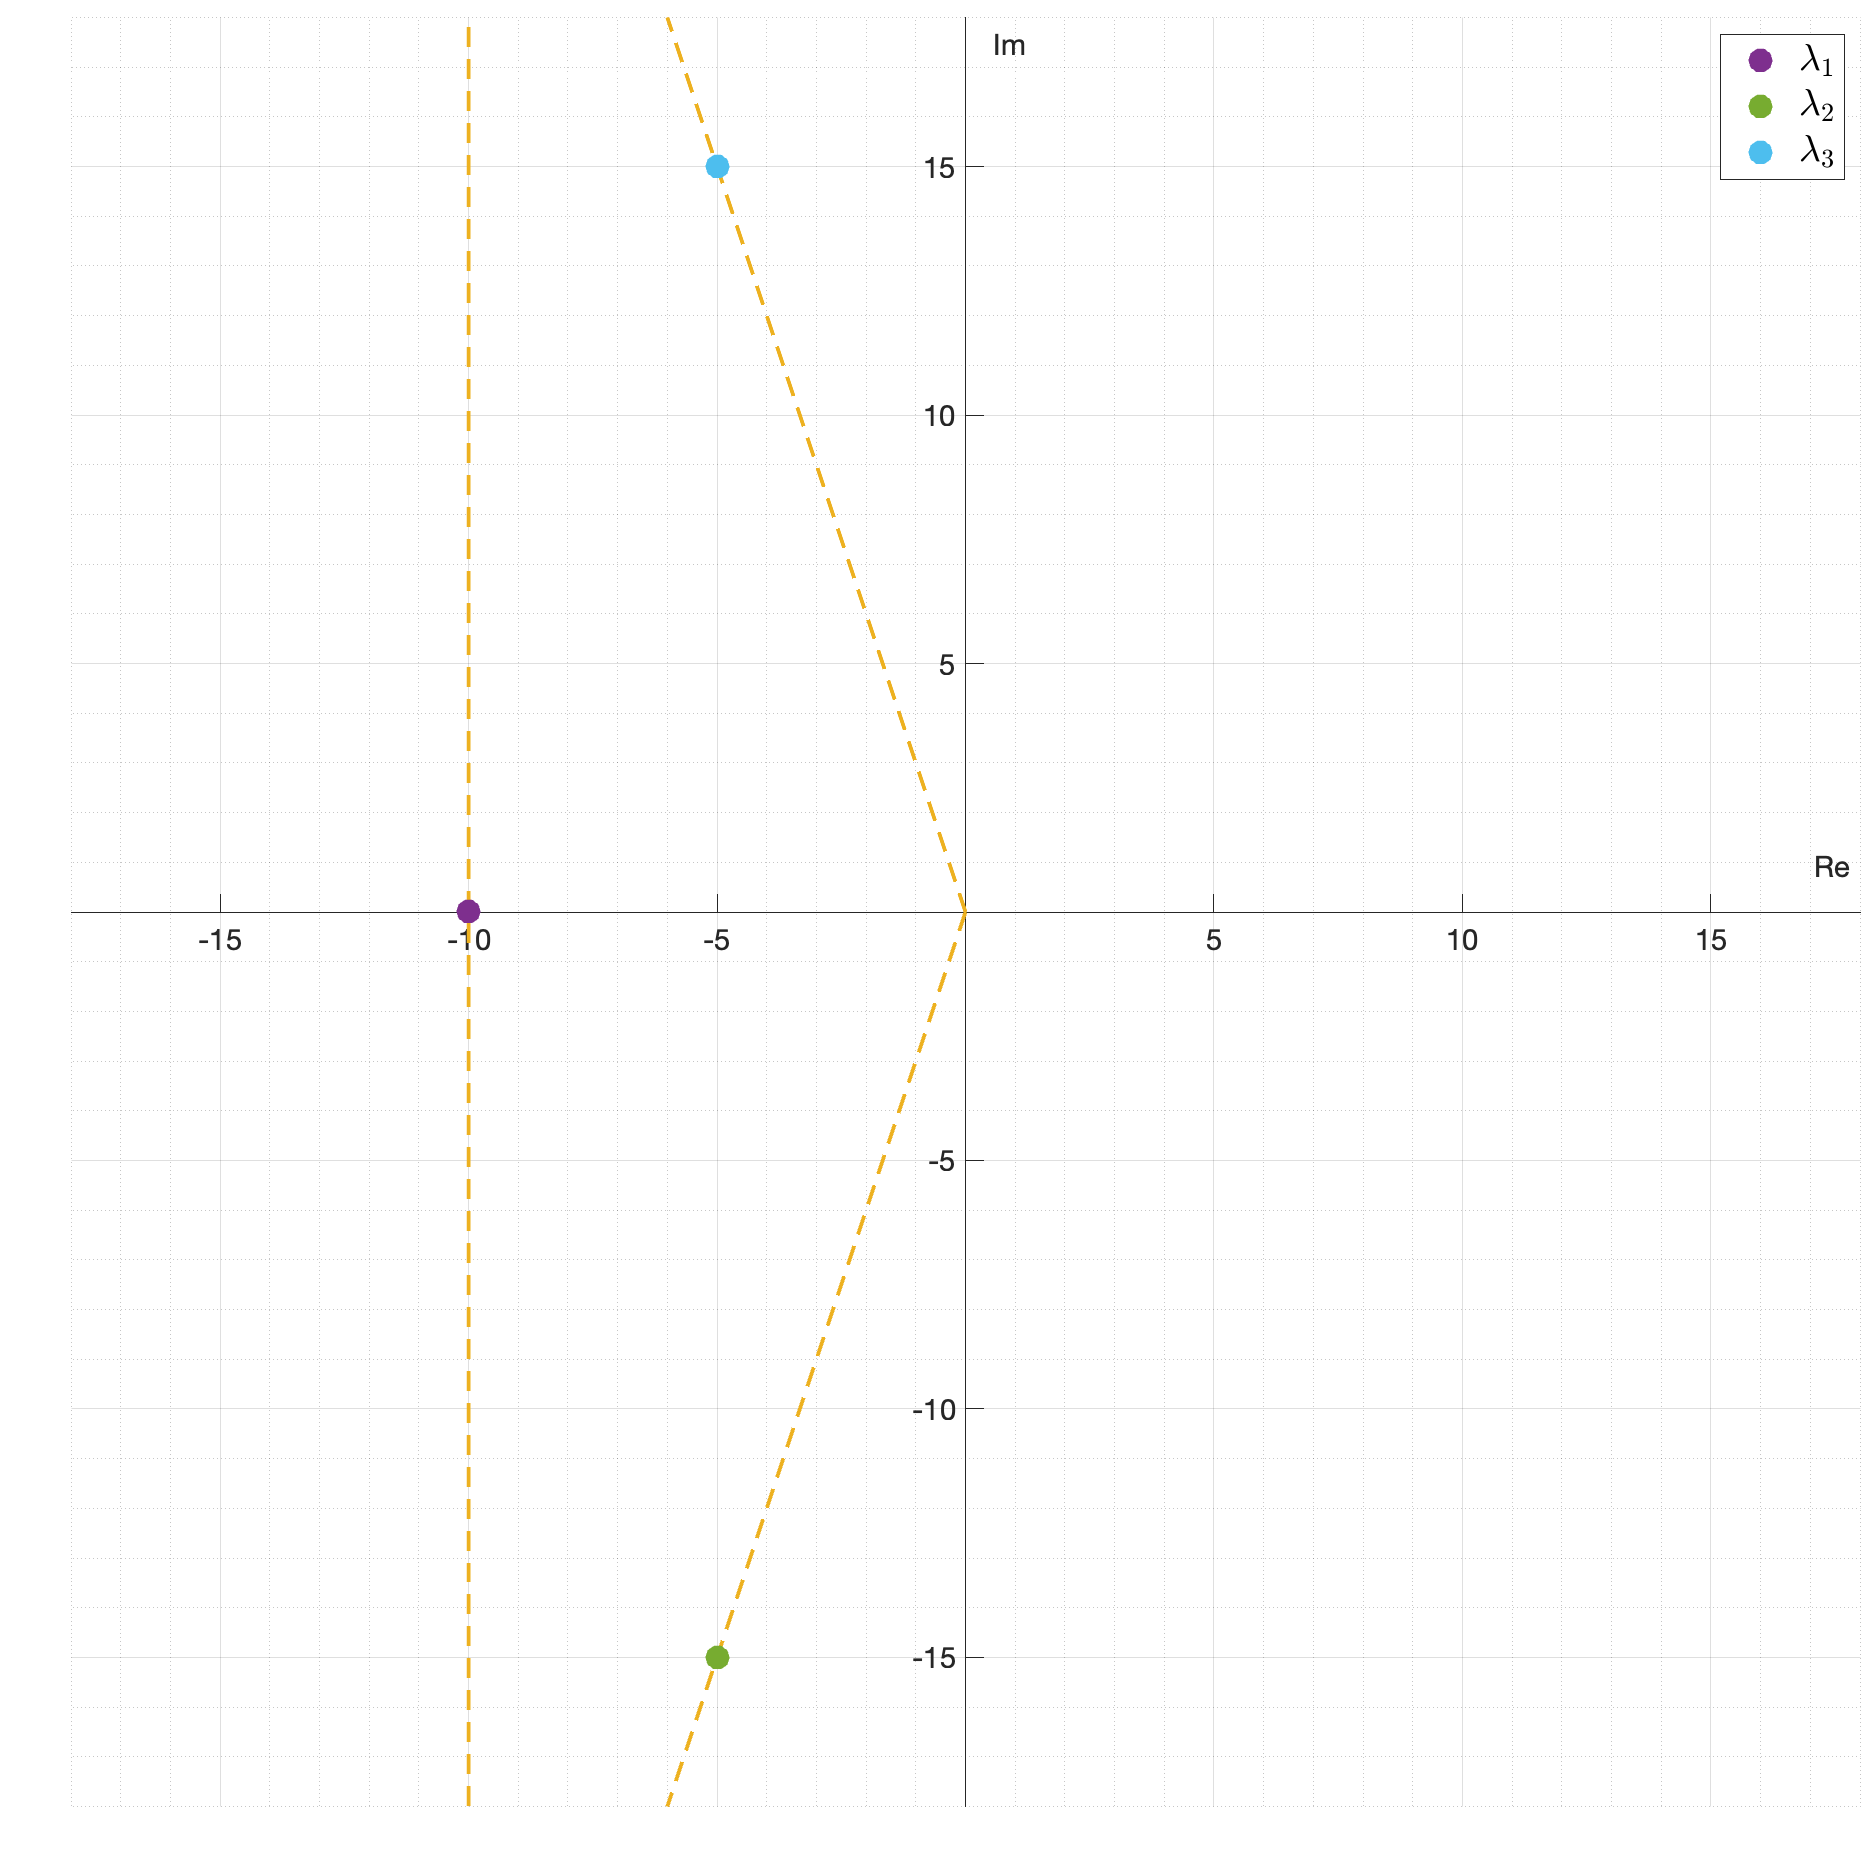
\includegraphics[width=0.8\textwidth]{media/plots/task2_points10.png}
    \caption{Расположение корней на комплексной плоскости в эксперименте 10}
    \label{fig:task_2_points10}
\end{figure}

\begin{figure}
    \centering
    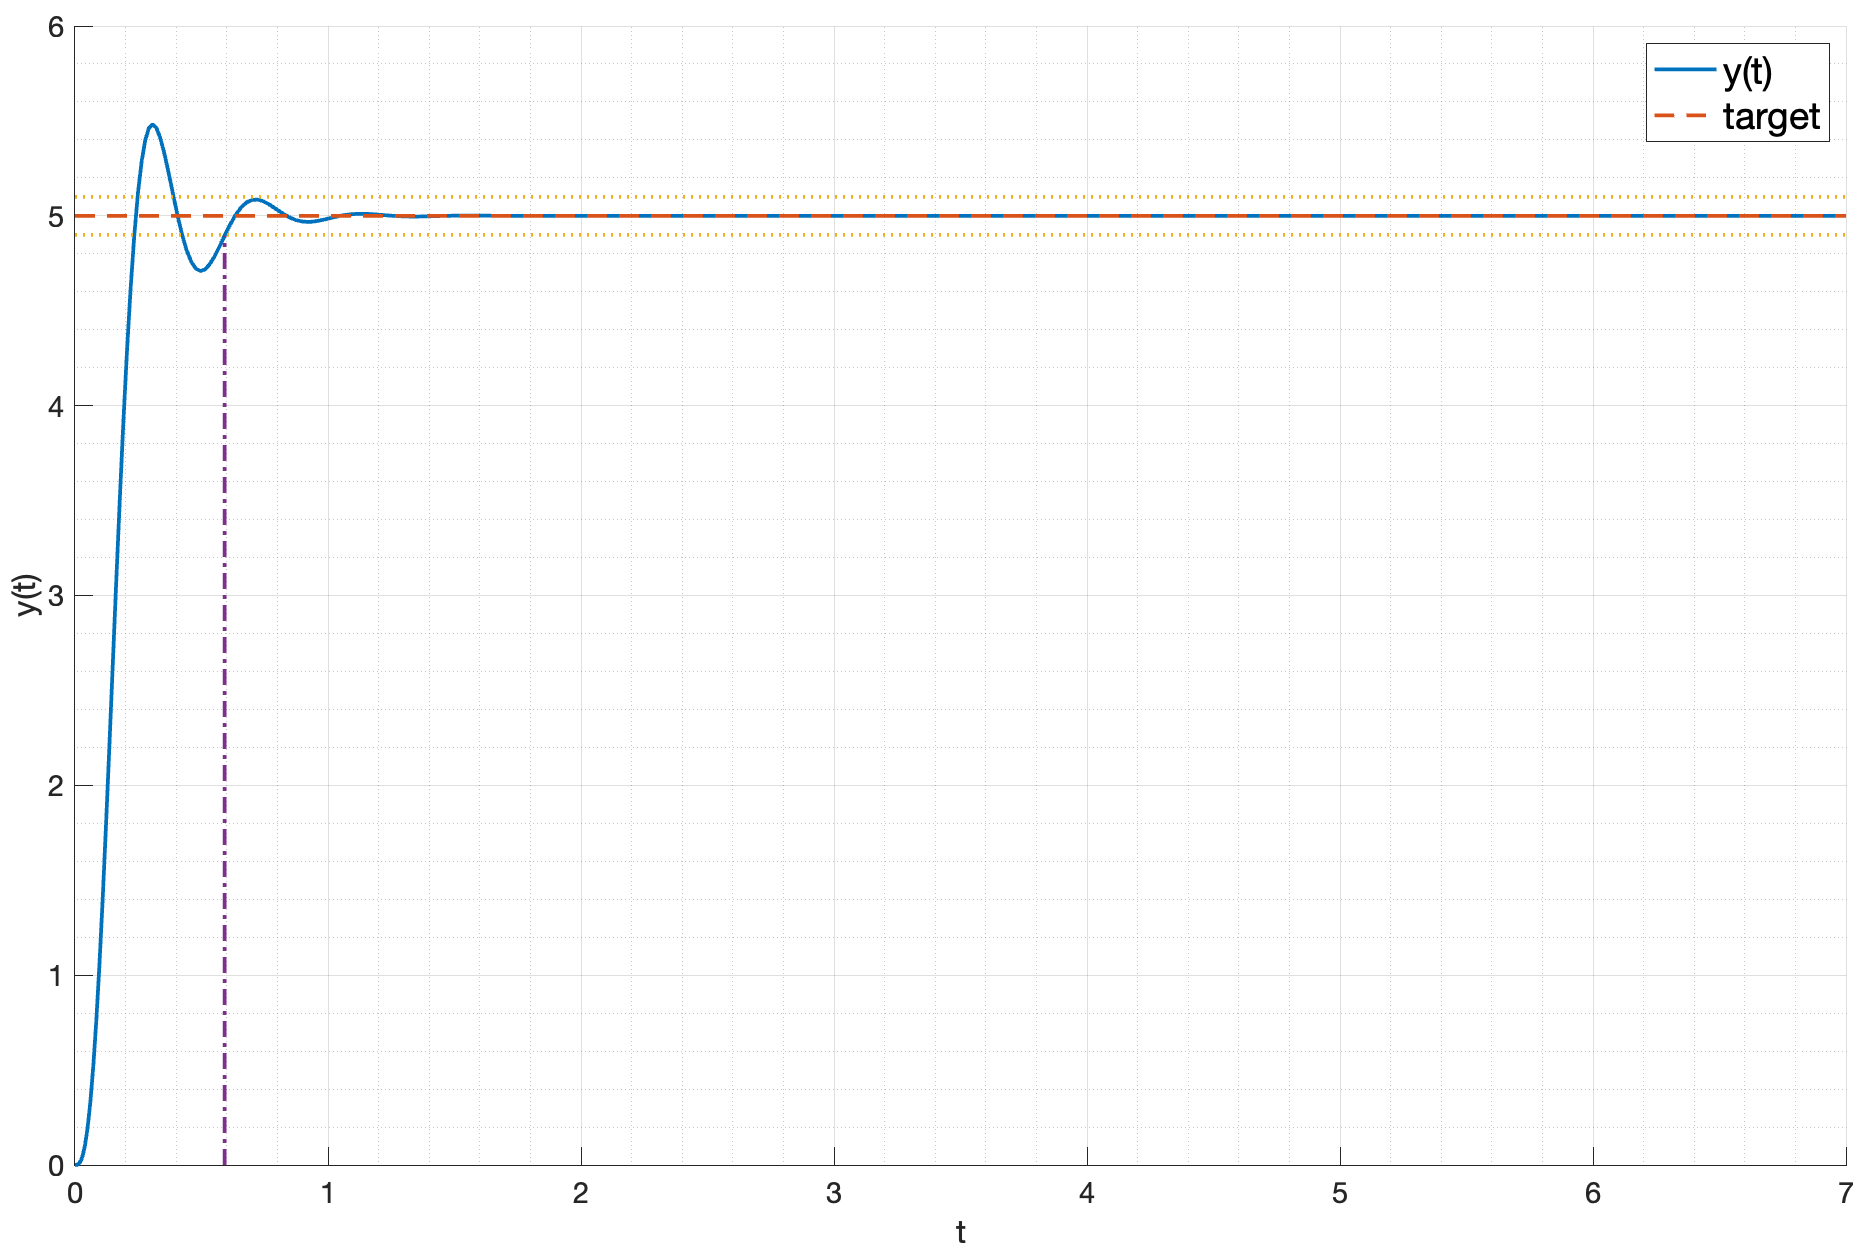
\includegraphics[width=\textwidth]{media/plots/task2_case10.png}
    \caption{Моделирование системы в эксперименте 10}
    \label{fig:task_2_case10}
\end{figure}

Время переходного процесса составило 0.59 секунды, перерегулирование 9\%.
Уменьшение времени переходного процесса и перерегулирования объясняется уменьшением
максимального значения действительной части корней характеристического уравнения, 
тем самым уменьшением угла наклона стороны трапеции и удаления правой границы от мнимой оси.

\FloatBarrier
\subsection{Вывод}
\begin{table}[ht!]
    \centering
    \begin{tabular}{|c|c|c|c|c|c|c|}
        \hline
        Номер & $\lambda_1$ & $\lambda_2$ & $\lambda_3$ & $T$ & $\sigma$ & Ссылка  \\
        \hline
        1 & -3 & -3 & -3 & 2.45 & 0 & \ref{task2_case1} \\
        \hline
        2 & -5 & -3 & -3 & 2.15 & 0 & \ref{task2_case2} \\
        \hline
        3 & -5 & -5 & -3 & 1.83 & 0 & \ref{task2_case3} \\
        \hline
        4 & -5 & -5 & -1 & 4.31 & 0 & \ref{task2_case4} \\
        \hline
        5 & -5 & -1 & -1 & 5.94 & 0 & \ref{task2_case5} \\
        \hline
        6 & -3 & -3-5i & -3+5i & 1.43 & 0 & \ref{task2_case6} \\
        \hline
        7 & -3 & -3-15i & -3+15i & 1.35 & 0 & \ref{task2_case7} \\
        \hline
        8 & -3 & -1-15i & -1+15i & 2.21 & 3.2 & \ref{task2_case8} \\
        \hline
        9 & -10 & -1-15i & -1+15i & 3.22 & 38 & \ref{task2_case9} \\
        \hline
        10 & -10 & -5-15i & -5+15i & 0.59 & 9 & \ref{task2_case10} \\
        \hline
    \end{tabular}
    \caption{Качество переходных процессов}
    \label{tab:quality}
\end{table}

В ходе моделирования систем с различными коэффициентами $\lambda_1$, $\lambda_2$, $\lambda_3$
были получены различные по качеству переходные процессы. В таблице \ref{tab:quality} приведены
результаты исследования. 

Можно сделать вывод, что теоретические предположения о зависимости времени переходного процесса
от максимального значения действительной части корней уравнения 
и перерегулирования от значения $\mu$ оказываются верными. В процессе моделирования не было 
обнаружено никаких аномалий, которые могли бы противоречить этим предположениям. Но и 
не было определено строгих зависимостей, так как каждый из параметров оказывает влияние на 
все характеристики переходного процесса. 

Для достижения максимального качества переходного процесса необходимо учитывать все параметры 
и подбирать их так, чтобы они взаимно компенсировали друг друга. 